\documentclass[licencjacka,en]{pracamgr}

\autor{Krzysztof Antoniak}{358985}
\autori{Michał Jadwiszczak}{406163}
\autorii{Jan Kukowski}{406204}
\autoriii{Maciej Procyk}{406304}

\title{Integrating Nussknacker with selected Machine Learning tools
}
\titlepl{Integracja projektu Nussknacker z wybranymi narzędziami Machine Learning
}

\kierunek{Computer Science}

\opiekun{mgr Grzegorz Grudziński\\
  Institute of Informatics\\
}

\date{June 2021}

% Socrates-Erasmus:
\dziedzina{11.3 Informatics, Computer Science}

% ACM
\klasyfikacja{
  \todo[inline]{Select codes from \href{https://dl.acm.org/ccs}{ACM Computing Classification System}}
}

\keywords{keywords, go, here
}

% Custom imports
\usepackage{forest}
\usepackage[unicode]{hyperref}
\usepackage{todonotes}
% End of custom imports

% Custom definitions
\newtheorem{definition}{Definition}[section]
% End of custom definitions

% Folder image for directory tree
\definecolor{folderbg}{RGB}{124,166,198}
\definecolor{folderborder}{RGB}{110,144,169}
\def\FolderSize{4pt}
\tikzset{
	folder/.pic={
		\filldraw[draw=folderborder,top color=folderbg!50,bottom color=folderbg]
		(-1.05*\FolderSize,0.2\FolderSize+5pt) rectangle ++(.75*\FolderSize,-0.2\FolderSize-5pt);
		\filldraw[draw=folderborder,top color=folderbg!50,bottom color=folderbg]
		(-1.15*\FolderSize,-\FolderSize) rectangle (1.15*\FolderSize,\FolderSize);
	}
}

\begin{document}
\maketitle

\begin{abstract}
  In the thesis we present a new implementation of Nussknacker's enricher named Prinz that is responsible for
Machine Learning models management and scoring. We describe the source of need for such implementation and
the background behind the Event Stream Processing approach. We show our approach to the process of developing
the open source library with API specification and our own API implementations including MLflow models
registry, PMML standard and H2O models registry. We describe the process towards managing open source project,
developers' environment management for the process of development and the decisions made to create our
implementation of Nussknacker’s enricher. Additionally, we present our thoughts on the topic of each integration,
its development process and the final results of API implementation which includes additional assumptions made
during the deployment of integration. As a final result of our work with the project, we provide working
library sources with readable examples of its deployment to the Nussknacker environment.

\end{abstract}

\tableofcontents
%\listoffigures
%\listoftables

% Chapters
\chapter*{Introduction}
\addcontentsline{toc}{chapter}{Introduction}

Introduction goes here.
\chapter{Architecture overview}
\label{chap:arch}

This chapter describes Prinz approach to integrating different tools with Nussknacker.
We will discuss our intermediate model representation in a typical process deployment.

Prinz extensions are injected to a Nussknacker instance in the configuration phase.
Instance administrator should configure model repositories which discover and provide model instances.
Each model is interpreted and exposed to Nussknacker UI as an enricher (see section \ref{sec:?}\todo{Link once we have it.}).
When Nussknacker process is deployed, Prinz translates parameters for the external model, delegates scoring and brings results back to the process.

\section{Model discovery}

Nussknacker configuration should use one or more instances of \texttt{ModelRepository}.
Repositories handle listing models available in configured storage.
Successful exchange with storage results in a list of model handles, which will be converted to enrichers.

Prinz comes with ready-to-use implementations using local filesystem or HTTP endpoint.
HTTP server is expected to expose list of models as JSON.
Developers can provide custom implementations of \texttt{ModelRepository}.

\section{Models}

Prinz uses an intermediate internal model representiation for unified handling of integrations.
\texttt{Model} trait represents a single entry in the Nussknacker UI.
Model is identified by name and may contain version info.
For some integrations it is possible to fetch metadata without loading the whole model.

By calling \texttt{Model.toModelInstance} system instantiates the model.
Exact behavior is implementation dependent, but this call should:
\begin{itemize}
	\item prepare model for signature extraction,
	\item prepare model for scoring.
\end{itemize}
Operation may require additional communication with the service.
At this point model would usually get loaded into memory if it is needed.

\subsection{Signatures}

Each machine learning model has inputs and outputs.
Their names (or ordering) along with data types form a model signature.
Since the range of supported types varies between different libraries, Prinz also abstracts signatures.

Each \texttt{ModelInstance} is instantiated with a signature provider, which will supply inputs and outputs of the model.
External data types are mapped to internal \texttt{SignatureType}s based on types supported by Nussknacker.
Extracted features and outputs are available in the Nussknacker UI for process designers.

\section{Scoring}

In a deployed Nussknacker process events move through the flow sequentially triggering computations at each step.
When computation reaches a Prinz enricher, it triggers scoring for supplied inputs.
(At this point system does not support batching).
Scoring starts by calling \texttt{run} on a \texttt{PrinzEnricher}.
During the scoring phase Prinz:
\begin{enumerate}
	\item converts inputs to external types based on the model signature,
	\item triggers scoring and receives outputs,
	\item translates results from external types to the ones used by Nussknacker.
\end{enumerate}
Received outputs may be used for further processing.

\chapter{MLflow integration}
\label{chap:mlflow}

\section{MLflow project overview}

MLflow is an open source project which allows managing the whole Machine Learning lifecycle.
It includes experimentation, deployment and reproducibility of models as well as a central registry
for versioning trained models. It was proposed by the Databricks team working with hundreds of companies
using Machine Learning as a solution to common production problems when working with Machine Learning
models and their deployment.

The whole MLflow platform was inspired by existing solutions from Facebook, Google and Uber which
seem to be limited because they support only a small set of built-in algorithms or a single library,
and they are strictly connected to each company’s infrastructure. They don’t allow easy use of new
Machine Learning libraries and share the results of work with an open community.

MLflow was designed to be an open source solution in two senses:

\begin{itemize}
	\item open source: it is an open source library publicly available that can be easily adapted
	by users and extended to expected form. Additionally, MLflow format makes it easy to share
	the whole workflow and models from one organization to another if you wish to share your
	code with collaborators.

	\item open interface: it is designed to work with many already available tools, Machine Learning
	libraries, implemented libraries and algorithms. It’s built using the REST APIs and readable data
	formats where for example a Machine Learning model can be seen as a single lambda function called
	on model evaluation. It was designed to be easily introduced to existing Machine Learning projects
	so the users can benefit from it immediately.
\end{itemize}

\section{Trained models management}

MLflow allows users to use existing models and easily convert them to open interface format.
When working with the MLflow framework we used the Python language for creating some Machine
Learning models for test purposes using the sklearn framework which is one of the many frameworks
supported by MLflow. Then the pretrained models were imported to MLflow repository which saved
their state in an external database and some data storage server that was responsible for keeping
the artefacts from training. In practice, the artefacts' data that was useful in our case was the
signature of the model which was exported to YAML file format.

The training process of used models was short enough that we can train the models every time the
MLflow server was created in a clean environment. This approach to creating this environment
allowed us to easily debug any inconsistency in models' training process because we could see
the difference between the clean environment and the environment with trained models.

\section{Trained models serving}

MLflow allows to deploy the trained models from its registry in a few ways including:
\begin{itemize}
	\item deploying \texttt{python\_function} model to Microsoft Azure ML
	\item deploying \texttt{python\_function} model to Amazon SageMaker
	\item exporting \texttt{python\_function} as an ApacheSpark UDF
	\item exporting a REST API endpoint serving the model as a docker image
	\item deploying the model as a REST API local server
\end{itemize}

Using any of these approaches may be easier or harder to deploy in practice depending on the architecture
that we already work with and the resources that can be used for the deployment process. Managing the local
REST API server is the easiest solution while it doesn’t scale up with the number of models. When the
developers take care about the environment, and it’s really hard to set up a fresh, clean environment
from scratch it’s better to manage the models using separated Docker containers (which deployment
process can additionally be easily automated).

In our environment the models after training are served as a local REST API in Docker image with MLflow
server inside where they have ports exposed for external usage. With this approach we can clean the
environment on every setup of integration tests of the library, download fresh, prepared images and
train the prepared models, which are then stored in MLflow clean database and S3 storage (that are
prepared as separate Docker images).

\section{MLflow Repository}

Configured MLflow server used in our environment model serves as the model registry which takes care
about model versioning and serving the base models' information using the REST API. As there is no
implementation for Scala (and Java) language for this REST API, we have created our own implementation
of the provided API with the usage of high level HTTP client library named sttp written by SoftwareMill
and the model objects serializer called circe powered by Cats. These two libraries allow us to create
the model corresponding to the official MLflow documentation which could be easily integrated with the
current version of MLflow models repository.

The whole model of data served by MLflow models registry server is provided in JSON format, for which
we managed to create corresponding models in code with the usage of compile time code analysis with
the Scala macros sbt plugin. In this approach it was enough to create the case classes with proper
fields to get automatic conversion between the received text data in JSON format and the objects
model in programming language. The whole process is based on JsonCondec code annotation which allows
to preprocess case classes in Scala in compile time and generate the Encoder and Decoder objects
implementations for the annotated class. In the standard approach the developer would have to manually
write this code which would just translate the JSON fields to object’s fields and vice versa while
this can be in most cases done automatically.

\section{MLflow Model and ModelInstance}

MLflow model is instantiated based on the data received and parsed in JSON format from MLflow models
registry and the signature data located in artefact storage of model. The signature data is parsed
separately from a YAML formatted file which is also mapped to JsonCodec model class with auto Encoder/Decoder
mechanism.

When the MLflow model is instantiated to allow scoring the served model, the whole conversion of data
sent to the external model service is done by the MLflow model instance during the run method invocation.
We created the abstract of Dataframe which corresponds to the single input for the model. When typed input
data comes from another Nussknacker service to the Prinz MLflow implementation, it has to be manually
converted to the valid JSON format, which can be determined based on the signature of the model. In the
runtime of the process the library receives the data in a unified format of type Any which then has to
be recognized and parsed before creating the input frame for the model. MLflow served models support two
types of JSON data providing named split and record orientations for compatibility and easier work with
different types of input data. In our model we use only a single approach of Dataframe to JSON conversion
as the data received from another service is always given in the same format. The data conversion process
which is needed before sending the data to the model and after receiving the data from the model was
implemented in the separated object’s MLFDataConverter methods as they don’t depend on the model and
exist in the model architecture as the static methods which are responsible only for data conversion
for this single type of implementation.

\section{MLflow Model Signature}

MLflow model signature is basically not a necessary part of a model registered in the models registry
provided by MLflow library. In our approach to the problem we assume that every user of our library
should save the models in the registry in the way which includes steps creating the model signature.
We found this way of typing the model input and output as the easiest one because the final user of
Nussknacker doesn’t have to know anything about model implementation (when it was logged to the registry
with a signature). Additionally creating the model with typed signature ensures the user that only the
valid input will be allowed for model input (which is not so obvious while the most of the models management
on the MLflow side is done with Python that hasn’t the static typing). However, creating the signature
for MLflow models in Python has a single drawback e.i. the model output doesn’t have any names and are
given as the ordered list in the JSON response. We manually create the additional labels for model outputs
in the process of scoring with the following outputs named \texttt{output\_0}, \texttt{output\_1} etc. Thanks to this
approach the final user of the Nussknacker GUI can configure the model in an easier way but still he has
to know the mapping between the interesting data and its order in the output model map.

It’s worth noting that the saved model signature in case of MLflow models is stored on external data
service like Amazon S3 data storage which seems to be the default choice of users of MLflow library.
In Prinz we implemented accessing the models’ signatures located only on S3 storage and here we see
the place for future improvements to provide some more generic approach of fetching the signature data.

\chapter{PMML integration}
\label{chap:pmml}

\section{PMML project overview}

Predictive Model Markup Language is a standard to represent predictive solutions.
It was developed by Dr. Robert Lee Grossman and the Data Mining Group.
The main goal was to be able to exchange predictive models produced by data mining
and machine learning algorithms between applications. The standard is widely spread across the world,
with over 30 organizations have announced their use of it.\cite{dmgpage}\cite{pmmlpowered}

In our Prinz solution, we are using \texttt{JPMML} library to serve PMML models. \texttt{JPMML} is open-source Java's
implementation of the PMML standard. This way we can support most of the standard versions, especially the latest
4.0, 4.1, 4.2, 4.3, and 4.4. Modules of the project used in Prinz are \texttt{JPMML-Model},
\texttt{JPMML-Evaluator} and \texttt{JPMML-Transpiler}. The first one is released under the terms and conditions
of the BSD 3-Clause "New" or "Revised" License. Model and transpiler are published under GNU Affero General Public License v3.0.
Therefore, that is the point of such license in PMML's package in our repo.\cite{jpmml}


\section{PMMML model representation}

PMML is based on XML language. The file is composed of several components such as:
\begin{itemize}
    \item header - contains general information about the document,
    \item data dictionary - contains definitions for fields used by the model,
    \item data transformations - maps user data into the form used by the mining model,
    \item model - contains the definition of the data mining model,
    \item mining schema - list of all fields used in the model. Can be a subset of fields defined in the data dictionary,
    \item targets - allows for post-processing of the predicted value. Can also be used for classification tasks,
    \item output - allows naming desired output fields expected from the model.
\end{itemize}


\section{PMML Repository}
\label{sec:pmml-repository}

The standard as well as its \texttt{JMPPL} implementation, does not provide any systematic way of versioning and serving models.
Thus, we had to design our way of storing PMML models. One of the project’s key principles was
to make Prinz open for further integrations and development. To ensure this we have implemented a \texttt{RepositoryClient}.
A generic API \texttt{AbstractRepositoryClient} provides methods to list files, open them and validate. Then the \texttt{RepositoryClientFactory}
knows which implementation of the client to choose based on URI’s schema. For now, we have supported the local filesystem client and HTTP client.
Working with a local file system repository is fairly straightforward. To get the HTTP repository to work, an HTML selector to a files' href elements
is required. Then if URI leads to HTML page, Prinz will download the page find the links to PMML files. Otherwise, if URI points
to the PMML file, the repository will simply get it.

To integrate a new one, you have to simply implement the abstract API and add one line to the factory’s registry.

As mentioned previously, \texttt{PMMLModelRepository} is based on \texttt{RepositoryClient}. By our convention,
the file name should be composed with model name and model version, separated by separator defined in the application’s config.
For instance, one of the PMML file's name in our GitHub repository is \texttt{PMML-FraudDetection-3-v0-1.pmml}, so it represents
\texttt{PMML-FraudDetection-3} model in version \texttt{0-1}.

\section{PMML Model and ModelInstance}

\texttt{PMMLModel}s are created based on the data received from scanning the path of the repository.
\texttt{RepositoryClient} returns payloads, where each of them contains basic information of models and input stream's source of a file.
Then the actual \texttt{PMMLRepository} creates models’ objects from that data.

\texttt{PMMLModel} holds the model’s name and its version. It is also responsible for providing a signature. The process of providing the signature will
be explained in short below.

\texttt{PMMLModelInstance} is using to create \texttt{PrinzEnricher}, which represents a tile on Nussknacker’s flow.
It is capable of actually running the model and mapping its output to be understood by Nussknacker.
We can achieve this, using an evaluator from \texttt{JPMML-Evaluator} library and passing the enricher's input to it.
The evaluator then takes care of actually running the model and returns the result.

\section{PMML Model Signature}

The PMML standard does not provide any separate method of retrieving the signature, rather than reading it from the file.
To get the input signature and also output signature we are using the previously mentioned evaluator from \texttt{JPMML-Evaluator} library.
Then \texttt{PMMLSignatureProvider} is converting each field of signature to the definition of fields properly typed in Prinz API
and parsing types to types supported by Nussknacker.
We are supporting most of the XMLSchema-2 types.

\chapter{Development environment}
\label{chap:devenv}

\section{Development environment overview}

We created a specially configured development environment as a part of our project repository to
simplify the process of the environment setup which is needed to run every integration with our
library and Nussknacker service. For this purpose a separate directory named \texttt{dev-environment} was
created which includes all the Docker configurations and scripts for setting up the environment
from scratch.

The base for configuration for the environment is made of the .env file which contains the environment
constant variables’ definitions and allows easily changing the ports of services and some paths in
Docker images that can be configured. This file is loaded also by the sbt which is then able to work
with the same environment for integration tests that use the Docker services to test
every integration.

The process of creating the new environment comes to running a single bash script from the \texttt{dev-environment}
which allows configuring the build process with additional flags specified for script execution. There is
a possibility to run only a single integration environment (e.g. only MLflow server repository with its
environment) or to exclude the process of library recompilation before placing it in the Nussknacker image.
All these improvements were added during the process of adding new integrations as we found it annoying
to spend a lot of time waiting for some part of the environment that wasn’t needed to test
and experiment with another integration. Additionally, we created the extra bash script for cleaning
the environment cached data as discovered to take a lot of disc space when having so many different
integrations with their environments in a single project.

Every integration has its \texttt{docker-compose} configuration file which specifies the Docker services
needed to run the integration environment. Additionally, there is a separate configuration named env
for Nussknacker image with its services, where the compiled Prinz library is placed. Thanks to
such an approach it is easier to set up every environment separately and run only the needed ones.
However, this also makes it a little harder to allow communication between every environment - we need
to manually add the Docker network to which the setup environments are connected during creation
time and then can communicate easily. Moreover, we decided not to expose every integration port for
external services for the other integrations and Nussknacker environment but create a single proxy
server for each integration which works as a barrier between the integration implementation details
and the outside world (and then the environment works more like in real life scenario).

The Docker images for each integration needs extra dependencies which are managed using the \texttt{conda}
environment manager. There is quite a lot of work to be done by installing all of them separately
so we decided to create the Docker images for integration and publish them in the external Docker
images repository. We decided to use the GitHub images hub which allows us to publish the images
as a part of our open-source project but unfortunately forces the user to log to GitHub before
downloading the image. However, this GitHub policy can change shortly as the community
doesn’t seem to like the logging requirement and there are many open discussions on this topic.

\section{Models serving in environment}

Every integration includes individual ways of models creating and serving them after the training process:

\begin{itemize}
    \item MLflow models are trained after creating the models' registry environment and then served as
    Docker services from the same Docker image. Their specification is saved on a separate PostgreSQL database and the signatures are kept on the S3 storage provided by the Minio Docker image. This setup
    makes the prepared environment behave like a production version of the MLflow server because there is no
    usage of local storage for data-keeping.

    \item PMML models are exported as the XML files during training on image start and served as the files by the HTTP little server written in Python. This approach uses the PMML Python dependencies only during
    training time as there is no alternative for models management server in case of PMML models representation.
    The models in our approach have to be listed in a specific way to give the developers ability to
    automatically find their locations with the proper selector path which specifies the models’ refs on the
    main site of the server and is configurable in Prinz.

    \item H2O server is somehow between the MLflow and the PMML integration as it sets up a full models registry server during training time and can list models and serve them with the usage of REST API. However, in our case, the simpler approach to H2O models was chosen and after training the models they are saved as the standard MOJO files and then led by the Prinz library as the local scoring models. Here we leave some room for future integrations as there is also a possibility to score the H2O models on the side of the H2O server like in the case of the MLflow registry.
\end{itemize}

\section{Proxying models environments}

For each integration, we created a separate proxy server based on light nginx alpine Docker image which
is set up with only a single configuration file having needed specifications. In the case of MLflow
integration, we tried to simulate the real-world scenario usage of the MLflow registry by manually setting
the proxy configuration connected with the buffering of the data and setting some custom requests’ headers.
In the other integration, the served models as the XML and MOJO files are only proxied with the change of
the port on which they are available to the user.

Furthermore, for each integration, the proxy also serves a few static files which contain the data needed
in the phase of integration tests. It is responsible for serving like some simple REST API server that
is capable of providing extra inputs for models in specific phases of library tests.

\section{Development environment in integration tests}

Each integration runs separately the integration tests which was one of the main reasons to separate
the environment configurations into a few files. During the tests phase there is a need to know the project
root file in the filesystem to locate these configuration files so before running any integration test
the user has to define the \texttt{REPOSITORY\_ABSOLUTE\_ROOT} environment variable. After this initial
configuration running tests from the console is as simple as calling a single sbt command as the whole
environment configuration is loaded with the sbt plugin from the \texttt{.env} file. However, in the case of the need
to run tests from an IDE, we need to specify separately the \texttt{.env} file in the test run configuration as for now
there is no possibility to load this information automatically in the IDE.

The testing phase includes testing the integration part e.i. scoring the models available in integration
models source and checking their signatures and other parameters. Moreover, there are tests which are
checking the models ability to being proxied with some external data source (outside of Nussknacker
environment source of data) so they use the described feature of nginx serving as a simple REST API
and use the local H2 database as the source of data for tests run. All of these described tests are
wrapped in the abstract traits specifications to allow running them on every integration with the minimal
configuration process. The process of running the tests for specific integration includes setting up the
environment from scratch but everything is done by the testcontainers library which uses the docker-compose
YAML files. This approach connects the source code of our library and its tests with the environment
definition while in the test running phase there is no need for the developer to manually set up the
environment. Additionally, the unit tests which don’t use the integrations’ environment just run scala
tests code without touching anything from the environment definition so there is an easy way to run them
and verify some specified parts of code without the process of working with any Docker containers.

\section{Development environment scheme}

The overview scheme of described development environment is presented below. It shows the scheme of
working with models via Nussknacker's frontend down to models listing and scoring models' instances.

\newpage
\scalebox{0.9}{\ifx\du\undefined
  \newlength{\du}
\fi
\setlength{\du}{15\unitlength}
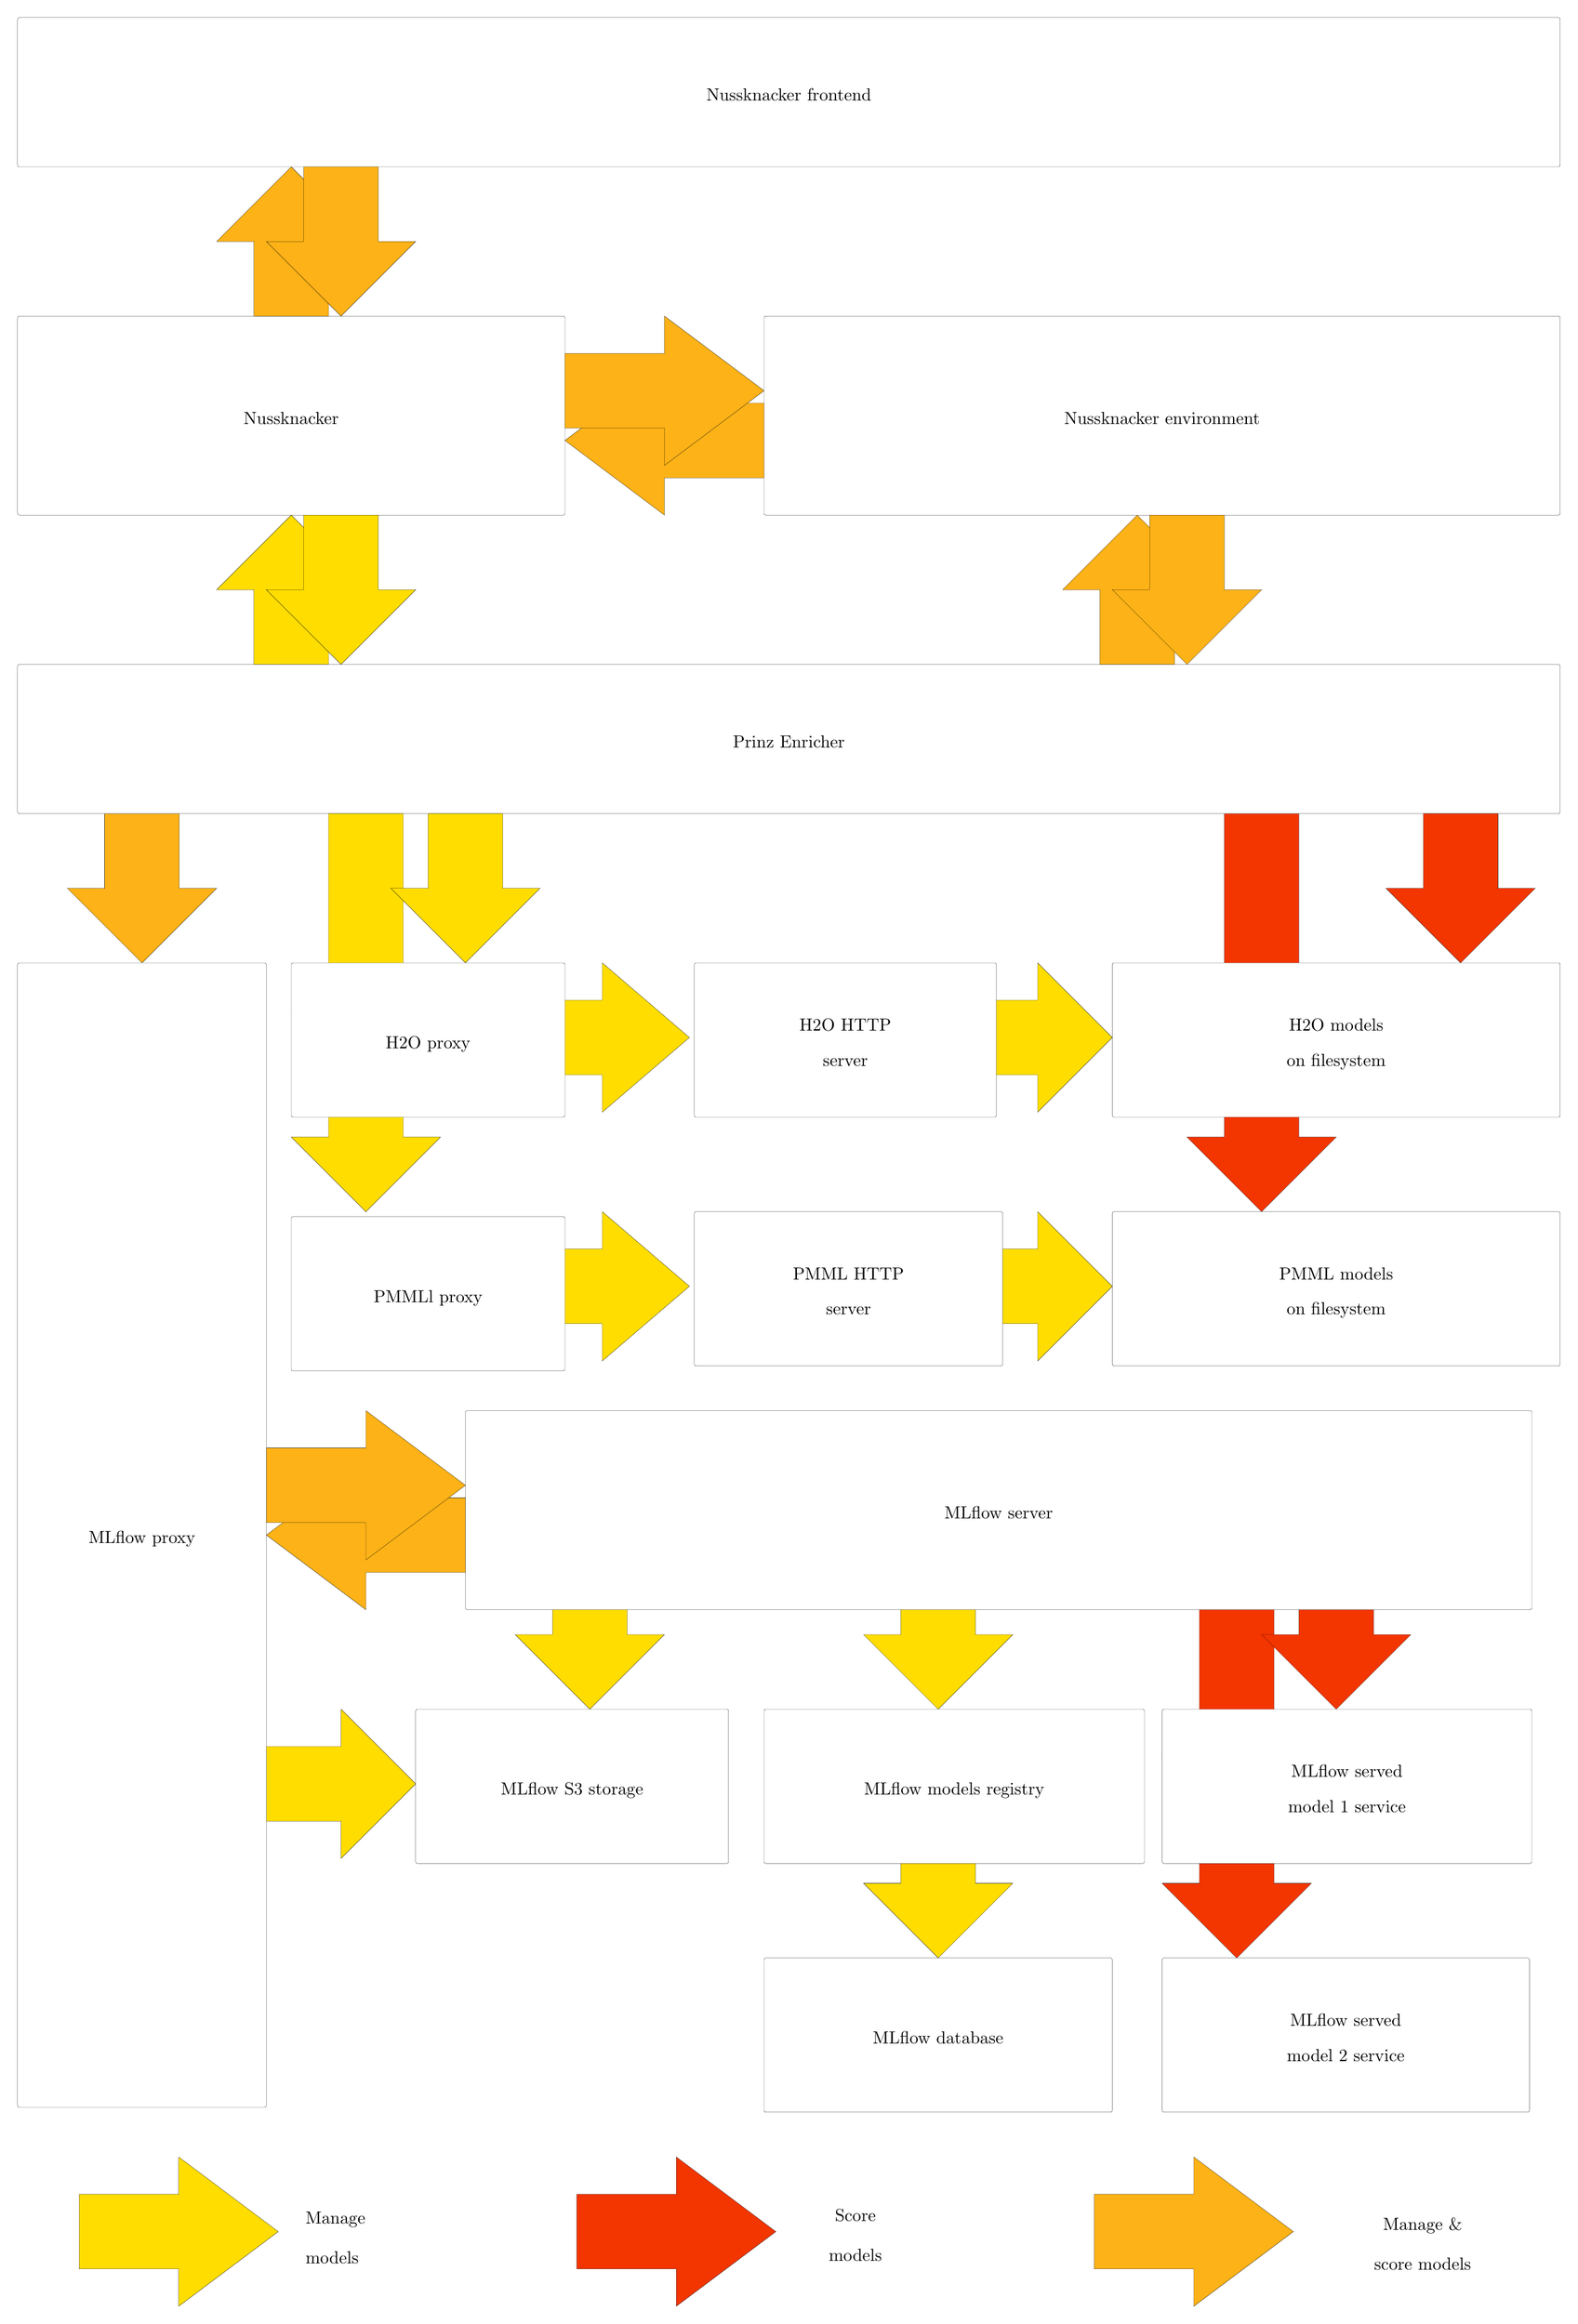
\begin{tikzpicture}[even odd rule]
\pgftransformxscale{1.000000}
\pgftransformyscale{-1.000000}
\definecolor{dialinecolor}{rgb}{0.000000, 0.000000, 0.000000}
\pgfsetstrokecolor{dialinecolor}
\pgfsetstrokeopacity{1.000000}
\definecolor{diafillcolor}{rgb}{1.000000, 1.000000, 1.000000}
\pgfsetfillcolor{diafillcolor}
\pgfsetfillopacity{1.000000}
\pgfsetlinewidth{0.100000\du}
\pgfsetdash{}{0pt}
\pgfsetbuttcap
\pgfsetmiterjoin
\pgfsetlinewidth{0.100000\du}
\pgfsetbuttcap
\pgfsetmiterjoin
\pgfsetdash{}{0pt}
\definecolor{diafillcolor}{rgb}{0.992157, 0.698039, 0.090196}
\pgfsetfillcolor{diafillcolor}
\pgfsetfillopacity{1.000000}
\fill (36.637500\du,52.750000\du)--(38.637500\du,52.750000\du)--(38.637500\du,52.000000\du)--(40.637500\du,53.500000\du)--(38.637500\du,55.000000\du)--(38.637500\du,54.250000\du)--(36.637500\du,54.250000\du)--cycle;
\definecolor{dialinecolor}{rgb}{0.000000, 0.000000, 0.000000}
\pgfsetstrokecolor{dialinecolor}
\pgfsetstrokeopacity{1.000000}
\draw (36.637500\du,52.750000\du)--(38.637500\du,52.750000\du)--(38.637500\du,52.000000\du)--(40.637500\du,53.500000\du)--(38.637500\du,55.000000\du)--(38.637500\du,54.250000\du)--(36.637500\du,54.250000\du)--cycle;
\pgfsetlinewidth{0.100000\du}
\pgfsetdash{}{0pt}
\pgfsetbuttcap
\pgfsetmiterjoin
\pgfsetlinewidth{0.100000\du}
\pgfsetbuttcap
\pgfsetmiterjoin
\pgfsetdash{}{0pt}
\definecolor{diafillcolor}{rgb}{0.952941, 0.207843, 0.000000}
\pgfsetfillcolor{diafillcolor}
\pgfsetfillopacity{1.000000}
\fill (26.237500\du,52.750000\du)--(28.237500\du,52.750000\du)--(28.237500\du,52.000000\du)--(30.237500\du,53.500000\du)--(28.237500\du,55.000000\du)--(28.237500\du,54.250000\du)--(26.237500\du,54.250000\du)--cycle;
\definecolor{dialinecolor}{rgb}{0.000000, 0.000000, 0.000000}
\pgfsetstrokecolor{dialinecolor}
\pgfsetstrokeopacity{1.000000}
\draw (26.237500\du,52.750000\du)--(28.237500\du,52.750000\du)--(28.237500\du,52.000000\du)--(30.237500\du,53.500000\du)--(28.237500\du,55.000000\du)--(28.237500\du,54.250000\du)--(26.237500\du,54.250000\du)--cycle;
\pgfsetlinewidth{0.100000\du}
\pgfsetdash{}{0pt}
\pgfsetbuttcap
\pgfsetmiterjoin
\pgfsetlinewidth{0.100000\du}
\pgfsetbuttcap
\pgfsetmiterjoin
\pgfsetdash{}{0pt}
\definecolor{diafillcolor}{rgb}{1.000000, 0.866667, 0.000000}
\pgfsetfillcolor{diafillcolor}
\pgfsetfillopacity{1.000000}
\fill (16.237500\du,52.750000\du)--(18.237500\du,52.750000\du)--(18.237500\du,52.000000\du)--(20.237500\du,53.500000\du)--(18.237500\du,55.000000\du)--(18.237500\du,54.250000\du)--(16.237500\du,54.250000\du)--cycle;
\definecolor{dialinecolor}{rgb}{0.000000, 0.000000, 0.000000}
\pgfsetstrokecolor{dialinecolor}
\pgfsetstrokeopacity{1.000000}
\draw (16.237500\du,52.750000\du)--(18.237500\du,52.750000\du)--(18.237500\du,52.000000\du)--(20.237500\du,53.500000\du)--(18.237500\du,55.000000\du)--(18.237500\du,54.250000\du)--(16.237500\du,54.250000\du)--cycle;
% setfont left to latex
\definecolor{dialinecolor}{rgb}{0.000000, 0.000000, 0.000000}
\pgfsetstrokecolor{dialinecolor}
\pgfsetstrokeopacity{1.000000}
\definecolor{diafillcolor}{rgb}{0.000000, 0.000000, 0.000000}
\pgfsetfillcolor{diafillcolor}
\pgfsetfillopacity{1.000000}
\node[anchor=base,inner sep=0pt, outer sep=0pt,color=dialinecolor] at (31.837500\du,53.300000\du){Score};
% setfont left to latex
\definecolor{dialinecolor}{rgb}{0.000000, 0.000000, 0.000000}
\pgfsetstrokecolor{dialinecolor}
\pgfsetstrokeopacity{1.000000}
\definecolor{diafillcolor}{rgb}{0.000000, 0.000000, 0.000000}
\pgfsetfillcolor{diafillcolor}
\pgfsetfillopacity{1.000000}
\node[anchor=base,inner sep=0pt, outer sep=0pt,color=dialinecolor] at (31.837500\du,54.100000\du){models};
% setfont left to latex
\definecolor{dialinecolor}{rgb}{0.000000, 0.000000, 0.000000}
\pgfsetstrokecolor{dialinecolor}
\pgfsetstrokeopacity{1.000000}
\definecolor{diafillcolor}{rgb}{0.000000, 0.000000, 0.000000}
\pgfsetfillcolor{diafillcolor}
\pgfsetfillopacity{1.000000}
\node[anchor=base west,inner sep=0pt,outer sep=0pt,color=dialinecolor] at (20.787500\du,53.350000\du){Manage};
% setfont left to latex
\definecolor{dialinecolor}{rgb}{0.000000, 0.000000, 0.000000}
\pgfsetstrokecolor{dialinecolor}
\pgfsetstrokeopacity{1.000000}
\definecolor{diafillcolor}{rgb}{0.000000, 0.000000, 0.000000}
\pgfsetfillcolor{diafillcolor}
\pgfsetfillopacity{1.000000}
\node[anchor=base west,inner sep=0pt,outer sep=0pt,color=dialinecolor] at (20.787500\du,54.150000\du){models};
% setfont left to latex
\definecolor{dialinecolor}{rgb}{0.000000, 0.000000, 0.000000}
\pgfsetstrokecolor{dialinecolor}
\pgfsetstrokeopacity{1.000000}
\definecolor{diafillcolor}{rgb}{0.000000, 0.000000, 0.000000}
\pgfsetfillcolor{diafillcolor}
\pgfsetfillopacity{1.000000}
\node[anchor=base,inner sep=0pt, outer sep=0pt,color=dialinecolor] at (43.237500\du,53.471250\du){Manage \& };
% setfont left to latex
\definecolor{dialinecolor}{rgb}{0.000000, 0.000000, 0.000000}
\pgfsetstrokecolor{dialinecolor}
\pgfsetstrokeopacity{1.000000}
\definecolor{diafillcolor}{rgb}{0.000000, 0.000000, 0.000000}
\pgfsetfillcolor{diafillcolor}
\pgfsetfillopacity{1.000000}
\node[anchor=base,inner sep=0pt, outer sep=0pt,color=dialinecolor] at (43.237500\du,54.271250\du){score models};
\pgfsetlinewidth{0.100000\du}
\pgfsetdash{}{0pt}
\pgfsetbuttcap
\pgfsetmiterjoin
\pgfsetlinewidth{0.100000\du}
\pgfsetbuttcap
\pgfsetmiterjoin
\pgfsetdash{}{0pt}
\definecolor{diafillcolor}{rgb}{0.992157, 0.698039, 0.090196}
\pgfsetfillcolor{diafillcolor}
\pgfsetfillopacity{1.000000}
\fill (16.750000\du,25.000000\du)--(16.750000\du,26.500000\du)--(16.000000\du,26.500000\du)--(17.500000\du,28.000000\du)--(19.000000\du,26.500000\du)--(18.250000\du,26.500000\du)--(18.250000\du,25.000000\du)--cycle;
\definecolor{dialinecolor}{rgb}{0.000000, 0.000000, 0.000000}
\pgfsetstrokecolor{dialinecolor}
\pgfsetstrokeopacity{1.000000}
\draw (16.750000\du,25.000000\du)--(16.750000\du,26.500000\du)--(16.000000\du,26.500000\du)--(17.500000\du,28.000000\du)--(19.000000\du,26.500000\du)--(18.250000\du,26.500000\du)--(18.250000\du,25.000000\du)--cycle;
\pgfsetlinewidth{0.100000\du}
\pgfsetdash{}{0pt}
\pgfsetbuttcap
\pgfsetmiterjoin
\pgfsetlinewidth{0.100000\du}
\pgfsetbuttcap
\pgfsetmiterjoin
\pgfsetdash{}{0pt}
\definecolor{diafillcolor}{rgb}{0.952941, 0.207843, 0.000000}
\pgfsetfillcolor{diafillcolor}
\pgfsetfillopacity{1.000000}
\fill (39.250000\du,25.000000\du)--(39.250000\du,29.000000\du)--(38.500000\du,29.000000\du)--(40.000000\du,33.000000\du)--(41.500000\du,29.000000\du)--(40.750000\du,29.000000\du)--(40.750000\du,25.000000\du)--cycle;
\definecolor{dialinecolor}{rgb}{0.000000, 0.000000, 0.000000}
\pgfsetstrokecolor{dialinecolor}
\pgfsetstrokeopacity{1.000000}
\draw (39.250000\du,25.000000\du)--(39.250000\du,29.000000\du)--(38.500000\du,29.000000\du)--(40.000000\du,33.000000\du)--(41.500000\du,29.000000\du)--(40.750000\du,29.000000\du)--(40.750000\du,25.000000\du)--cycle;
\pgfsetlinewidth{0.100000\du}
\pgfsetdash{}{0pt}
\pgfsetbuttcap
\pgfsetmiterjoin
\pgfsetlinewidth{0.100000\du}
\pgfsetbuttcap
\pgfsetmiterjoin
\pgfsetdash{}{0pt}
\definecolor{diafillcolor}{rgb}{0.952941, 0.207843, 0.000000}
\pgfsetfillcolor{diafillcolor}
\pgfsetfillopacity{1.000000}
\fill (39.250000\du,30.000000\du)--(39.250000\du,31.500000\du)--(38.500000\du,31.500000\du)--(40.000000\du,33.000000\du)--(41.500000\du,31.500000\du)--(40.750000\du,31.500000\du)--(40.750000\du,30.000000\du)--cycle;
\definecolor{dialinecolor}{rgb}{0.000000, 0.000000, 0.000000}
\pgfsetstrokecolor{dialinecolor}
\pgfsetstrokeopacity{1.000000}
\draw (39.250000\du,30.000000\du)--(39.250000\du,31.500000\du)--(38.500000\du,31.500000\du)--(40.000000\du,33.000000\du)--(41.500000\du,31.500000\du)--(40.750000\du,31.500000\du)--(40.750000\du,30.000000\du)--cycle;
\pgfsetlinewidth{0.100000\du}
\pgfsetdash{}{0pt}
\pgfsetmiterjoin
{\pgfsetcornersarced{\pgfpoint{1.000000\du}{1.000000\du}}\definecolor{diafillcolor}{rgb}{1.000000, 1.000000, 1.000000}
\pgfsetfillcolor{diafillcolor}
\pgfsetfillopacity{1.000000}
\fill (23.000000\du,43.000000\du)--(23.000000\du,46.100000\du)--(29.287500\du,46.100000\du)--(29.287500\du,43.000000\du)--cycle;
}{\pgfsetcornersarced{\pgfpoint{1.000000\du}{1.000000\du}}\definecolor{dialinecolor}{rgb}{0.000000, 0.000000, 0.000000}
\pgfsetstrokecolor{dialinecolor}
\pgfsetstrokeopacity{1.000000}
\draw (23.000000\du,43.000000\du)--(23.000000\du,46.100000\du)--(29.287500\du,46.100000\du)--(29.287500\du,43.000000\du)--cycle;
}% setfont left to latex
\definecolor{dialinecolor}{rgb}{0.000000, 0.000000, 0.000000}
\pgfsetstrokecolor{dialinecolor}
\pgfsetstrokeopacity{1.000000}
\definecolor{diafillcolor}{rgb}{0.000000, 0.000000, 0.000000}
\pgfsetfillcolor{diafillcolor}
\pgfsetfillopacity{1.000000}
\node[anchor=base,inner sep=0pt, outer sep=0pt,color=dialinecolor] at (26.143750\du,44.722222\du){MLflow S3 storage};
\pgfsetlinewidth{0.100000\du}
\pgfsetdash{}{0pt}
\pgfsetmiterjoin
{\pgfsetcornersarced{\pgfpoint{1.000000\du}{1.000000\du}}\definecolor{diafillcolor}{rgb}{1.000000, 1.000000, 1.000000}
\pgfsetfillcolor{diafillcolor}
\pgfsetfillopacity{1.000000}
\fill (30.000000\du,48.000000\du)--(30.000000\du,51.100000\du)--(37.000000\du,51.100000\du)--(37.000000\du,48.000000\du)--cycle;
}{\pgfsetcornersarced{\pgfpoint{1.000000\du}{1.000000\du}}\definecolor{dialinecolor}{rgb}{0.000000, 0.000000, 0.000000}
\pgfsetstrokecolor{dialinecolor}
\pgfsetstrokeopacity{1.000000}
\draw (30.000000\du,48.000000\du)--(30.000000\du,51.100000\du)--(37.000000\du,51.100000\du)--(37.000000\du,48.000000\du)--cycle;
}% setfont left to latex
\definecolor{dialinecolor}{rgb}{0.000000, 0.000000, 0.000000}
\pgfsetstrokecolor{dialinecolor}
\pgfsetstrokeopacity{1.000000}
\definecolor{diafillcolor}{rgb}{0.000000, 0.000000, 0.000000}
\pgfsetfillcolor{diafillcolor}
\pgfsetfillopacity{1.000000}
\node[anchor=base,inner sep=0pt, outer sep=0pt,color=dialinecolor] at (33.500000\du,49.722222\du){MLflow database};
\pgfsetlinewidth{0.100000\du}
\pgfsetdash{}{0pt}
\pgfsetbuttcap
\pgfsetmiterjoin
\pgfsetlinewidth{0.100000\du}
\pgfsetbuttcap
\pgfsetmiterjoin
\pgfsetdash{}{0pt}
\definecolor{diafillcolor}{rgb}{1.000000, 0.866667, 0.000000}
\pgfsetfillcolor{diafillcolor}
\pgfsetfillopacity{1.000000}
\fill (32.750000\du,45.000000\du)--(32.750000\du,46.500000\du)--(32.000000\du,46.500000\du)--(33.500000\du,48.000000\du)--(35.000000\du,46.500000\du)--(34.250000\du,46.500000\du)--(34.250000\du,45.000000\du)--cycle;
\definecolor{dialinecolor}{rgb}{0.000000, 0.000000, 0.000000}
\pgfsetstrokecolor{dialinecolor}
\pgfsetstrokeopacity{1.000000}
\draw (32.750000\du,45.000000\du)--(32.750000\du,46.500000\du)--(32.000000\du,46.500000\du)--(33.500000\du,48.000000\du)--(35.000000\du,46.500000\du)--(34.250000\du,46.500000\du)--(34.250000\du,45.000000\du)--cycle;
\pgfsetlinewidth{0.100000\du}
\pgfsetdash{}{0pt}
\pgfsetbuttcap
\pgfsetmiterjoin
\pgfsetlinewidth{0.100000\du}
\pgfsetbuttcap
\pgfsetmiterjoin
\pgfsetdash{}{0pt}
\definecolor{diafillcolor}{rgb}{0.952941, 0.207843, 0.000000}
\pgfsetfillcolor{diafillcolor}
\pgfsetfillopacity{1.000000}
\fill (38.750000\du,40.000000\du)--(38.750000\du,44.000000\du)--(38.000000\du,44.000000\du)--(39.500000\du,48.000000\du)--(41.000000\du,44.000000\du)--(40.250000\du,44.000000\du)--(40.250000\du,40.000000\du)--cycle;
\definecolor{dialinecolor}{rgb}{0.000000, 0.000000, 0.000000}
\pgfsetstrokecolor{dialinecolor}
\pgfsetstrokeopacity{1.000000}
\draw (38.750000\du,40.000000\du)--(38.750000\du,44.000000\du)--(38.000000\du,44.000000\du)--(39.500000\du,48.000000\du)--(41.000000\du,44.000000\du)--(40.250000\du,44.000000\du)--(40.250000\du,40.000000\du)--cycle;
\pgfsetlinewidth{0.100000\du}
\pgfsetdash{}{0pt}
\pgfsetbuttcap
\pgfsetmiterjoin
\pgfsetlinewidth{0.100000\du}
\pgfsetbuttcap
\pgfsetmiterjoin
\pgfsetdash{}{0pt}
\definecolor{diafillcolor}{rgb}{0.952941, 0.207843, 0.000000}
\pgfsetfillcolor{diafillcolor}
\pgfsetfillopacity{1.000000}
\fill (38.750000\du,45.000000\du)--(38.750000\du,46.500000\du)--(38.000000\du,46.500000\du)--(39.500000\du,48.000000\du)--(41.000000\du,46.500000\du)--(40.250000\du,46.500000\du)--(40.250000\du,45.000000\du)--cycle;
\definecolor{dialinecolor}{rgb}{0.000000, 0.000000, 0.000000}
\pgfsetstrokecolor{dialinecolor}
\pgfsetstrokeopacity{1.000000}
\draw (38.750000\du,45.000000\du)--(38.750000\du,46.500000\du)--(38.000000\du,46.500000\du)--(39.500000\du,48.000000\du)--(41.000000\du,46.500000\du)--(40.250000\du,46.500000\du)--(40.250000\du,45.000000\du)--cycle;
\pgfsetlinewidth{0.100000\du}
\pgfsetdash{}{0pt}
\pgfsetmiterjoin
{\pgfsetcornersarced{\pgfpoint{1.000000\du}{1.000000\du}}\definecolor{diafillcolor}{rgb}{1.000000, 1.000000, 1.000000}
\pgfsetfillcolor{diafillcolor}
\pgfsetfillopacity{1.000000}
\fill (38.000000\du,43.000000\du)--(38.000000\du,46.100000\du)--(45.431875\du,46.100000\du)--(45.431875\du,43.000000\du)--cycle;
}{\pgfsetcornersarced{\pgfpoint{1.000000\du}{1.000000\du}}\definecolor{dialinecolor}{rgb}{0.000000, 0.000000, 0.000000}
\pgfsetstrokecolor{dialinecolor}
\pgfsetstrokeopacity{1.000000}
\draw (38.000000\du,43.000000\du)--(38.000000\du,46.100000\du)--(45.431875\du,46.100000\du)--(45.431875\du,43.000000\du)--cycle;
}% setfont left to latex
\definecolor{dialinecolor}{rgb}{0.000000, 0.000000, 0.000000}
\pgfsetstrokecolor{dialinecolor}
\pgfsetstrokeopacity{1.000000}
\definecolor{diafillcolor}{rgb}{0.000000, 0.000000, 0.000000}
\pgfsetfillcolor{diafillcolor}
\pgfsetfillopacity{1.000000}
\node[anchor=base,inner sep=0pt, outer sep=0pt,color=dialinecolor] at (41.715938\du,44.369444\du){MLflow served };
% setfont left to latex
\definecolor{dialinecolor}{rgb}{0.000000, 0.000000, 0.000000}
\pgfsetstrokecolor{dialinecolor}
\pgfsetstrokeopacity{1.000000}
\definecolor{diafillcolor}{rgb}{0.000000, 0.000000, 0.000000}
\pgfsetfillcolor{diafillcolor}
\pgfsetfillopacity{1.000000}
\node[anchor=base,inner sep=0pt, outer sep=0pt,color=dialinecolor] at (41.715938\du,45.075000\du){model 1 service};
\pgfsetlinewidth{0.100000\du}
\pgfsetdash{}{0pt}
\pgfsetbuttcap
\pgfsetmiterjoin
\pgfsetlinewidth{0.100000\du}
\pgfsetbuttcap
\pgfsetmiterjoin
\pgfsetdash{}{0pt}
\definecolor{diafillcolor}{rgb}{0.952941, 0.207843, 0.000000}
\pgfsetfillcolor{diafillcolor}
\pgfsetfillopacity{1.000000}
\fill (40.750000\du,40.000000\du)--(40.750000\du,41.500000\du)--(40.000000\du,41.500000\du)--(41.500000\du,43.000000\du)--(43.000000\du,41.500000\du)--(42.250000\du,41.500000\du)--(42.250000\du,40.000000\du)--cycle;
\definecolor{dialinecolor}{rgb}{0.000000, 0.000000, 0.000000}
\pgfsetstrokecolor{dialinecolor}
\pgfsetstrokeopacity{1.000000}
\draw (40.750000\du,40.000000\du)--(40.750000\du,41.500000\du)--(40.000000\du,41.500000\du)--(41.500000\du,43.000000\du)--(43.000000\du,41.500000\du)--(42.250000\du,41.500000\du)--(42.250000\du,40.000000\du)--cycle;
\pgfsetlinewidth{0.100000\du}
\pgfsetdash{}{0pt}
\pgfsetmiterjoin
{\pgfsetcornersarced{\pgfpoint{1.000000\du}{1.000000\du}}\definecolor{diafillcolor}{rgb}{1.000000, 1.000000, 1.000000}
\pgfsetfillcolor{diafillcolor}
\pgfsetfillopacity{1.000000}
\fill (38.000000\du,48.000000\du)--(38.000000\du,51.100000\du)--(45.381875\du,51.100000\du)--(45.381875\du,48.000000\du)--cycle;
}{\pgfsetcornersarced{\pgfpoint{1.000000\du}{1.000000\du}}\definecolor{dialinecolor}{rgb}{0.000000, 0.000000, 0.000000}
\pgfsetstrokecolor{dialinecolor}
\pgfsetstrokeopacity{1.000000}
\draw (38.000000\du,48.000000\du)--(38.000000\du,51.100000\du)--(45.381875\du,51.100000\du)--(45.381875\du,48.000000\du)--cycle;
}% setfont left to latex
\definecolor{dialinecolor}{rgb}{0.000000, 0.000000, 0.000000}
\pgfsetstrokecolor{dialinecolor}
\pgfsetstrokeopacity{1.000000}
\definecolor{diafillcolor}{rgb}{0.000000, 0.000000, 0.000000}
\pgfsetfillcolor{diafillcolor}
\pgfsetfillopacity{1.000000}
\node[anchor=base,inner sep=0pt, outer sep=0pt,color=dialinecolor] at (41.690938\du,49.369444\du){MLflow served };
% setfont left to latex
\definecolor{dialinecolor}{rgb}{0.000000, 0.000000, 0.000000}
\pgfsetstrokecolor{dialinecolor}
\pgfsetstrokeopacity{1.000000}
\definecolor{diafillcolor}{rgb}{0.000000, 0.000000, 0.000000}
\pgfsetfillcolor{diafillcolor}
\pgfsetfillopacity{1.000000}
\node[anchor=base,inner sep=0pt, outer sep=0pt,color=dialinecolor] at (41.690938\du,50.075000\du){model 2 service};
\pgfsetlinewidth{0.100000\du}
\pgfsetdash{}{0pt}
\pgfsetbuttcap
\pgfsetmiterjoin
\pgfsetlinewidth{0.100000\du}
\pgfsetbuttcap
\pgfsetmiterjoin
\pgfsetdash{}{0pt}
\definecolor{diafillcolor}{rgb}{1.000000, 0.866667, 0.000000}
\pgfsetfillcolor{diafillcolor}
\pgfsetfillopacity{1.000000}
\fill (32.750000\du,40.000000\du)--(32.750000\du,41.500000\du)--(32.000000\du,41.500000\du)--(33.500000\du,43.000000\du)--(35.000000\du,41.500000\du)--(34.250000\du,41.500000\du)--(34.250000\du,40.000000\du)--cycle;
\definecolor{dialinecolor}{rgb}{0.000000, 0.000000, 0.000000}
\pgfsetstrokecolor{dialinecolor}
\pgfsetstrokeopacity{1.000000}
\draw (32.750000\du,40.000000\du)--(32.750000\du,41.500000\du)--(32.000000\du,41.500000\du)--(33.500000\du,43.000000\du)--(35.000000\du,41.500000\du)--(34.250000\du,41.500000\du)--(34.250000\du,40.000000\du)--cycle;
\pgfsetlinewidth{0.100000\du}
\pgfsetdash{}{0pt}
\pgfsetmiterjoin
{\pgfsetcornersarced{\pgfpoint{1.000000\du}{1.000000\du}}\definecolor{diafillcolor}{rgb}{1.000000, 1.000000, 1.000000}
\pgfsetfillcolor{diafillcolor}
\pgfsetfillopacity{1.000000}
\fill (30.000000\du,43.000000\du)--(30.000000\du,46.100000\du)--(37.645000\du,46.100000\du)--(37.645000\du,43.000000\du)--cycle;
}{\pgfsetcornersarced{\pgfpoint{1.000000\du}{1.000000\du}}\definecolor{dialinecolor}{rgb}{0.000000, 0.000000, 0.000000}
\pgfsetstrokecolor{dialinecolor}
\pgfsetstrokeopacity{1.000000}
\draw (30.000000\du,43.000000\du)--(30.000000\du,46.100000\du)--(37.645000\du,46.100000\du)--(37.645000\du,43.000000\du)--cycle;
}% setfont left to latex
\definecolor{dialinecolor}{rgb}{0.000000, 0.000000, 0.000000}
\pgfsetstrokecolor{dialinecolor}
\pgfsetstrokeopacity{1.000000}
\definecolor{diafillcolor}{rgb}{0.000000, 0.000000, 0.000000}
\pgfsetfillcolor{diafillcolor}
\pgfsetfillopacity{1.000000}
\node[anchor=base,inner sep=0pt, outer sep=0pt,color=dialinecolor] at (33.822500\du,44.722222\du){MLflow models registry};
\pgfsetlinewidth{0.100000\du}
\pgfsetdash{}{0pt}
\pgfsetbuttcap
\pgfsetmiterjoin
\pgfsetlinewidth{0.100000\du}
\pgfsetbuttcap
\pgfsetmiterjoin
\pgfsetdash{}{0pt}
\definecolor{diafillcolor}{rgb}{1.000000, 0.866667, 0.000000}
\pgfsetfillcolor{diafillcolor}
\pgfsetfillopacity{1.000000}
\fill (25.750000\du,40.000000\du)--(25.750000\du,41.500000\du)--(25.000000\du,41.500000\du)--(26.500000\du,43.000000\du)--(28.000000\du,41.500000\du)--(27.250000\du,41.500000\du)--(27.250000\du,40.000000\du)--cycle;
\definecolor{dialinecolor}{rgb}{0.000000, 0.000000, 0.000000}
\pgfsetstrokecolor{dialinecolor}
\pgfsetstrokeopacity{1.000000}
\draw (25.750000\du,40.000000\du)--(25.750000\du,41.500000\du)--(25.000000\du,41.500000\du)--(26.500000\du,43.000000\du)--(28.000000\du,41.500000\du)--(27.250000\du,41.500000\du)--(27.250000\du,40.000000\du)--cycle;
\pgfsetlinewidth{0.100000\du}
\pgfsetdash{}{0pt}
\pgfsetmiterjoin
{\pgfsetcornersarced{\pgfpoint{1.000000\du}{1.000000\du}}\definecolor{diafillcolor}{rgb}{1.000000, 1.000000, 1.000000}
\pgfsetfillcolor{diafillcolor}
\pgfsetfillopacity{1.000000}
\fill (24.000000\du,37.000000\du)--(24.000000\du,41.000000\du)--(45.431875\du,41.000000\du)--(45.431875\du,37.000000\du)--cycle;
}{\pgfsetcornersarced{\pgfpoint{1.000000\du}{1.000000\du}}\definecolor{dialinecolor}{rgb}{0.000000, 0.000000, 0.000000}
\pgfsetstrokecolor{dialinecolor}
\pgfsetstrokeopacity{1.000000}
\draw (24.000000\du,37.000000\du)--(24.000000\du,41.000000\du)--(45.431875\du,41.000000\du)--(45.431875\du,37.000000\du)--cycle;
}% setfont left to latex
\definecolor{dialinecolor}{rgb}{0.000000, 0.000000, 0.000000}
\pgfsetstrokecolor{dialinecolor}
\pgfsetstrokeopacity{1.000000}
\definecolor{diafillcolor}{rgb}{0.000000, 0.000000, 0.000000}
\pgfsetfillcolor{diafillcolor}
\pgfsetfillopacity{1.000000}
\node[anchor=base,inner sep=0pt, outer sep=0pt,color=dialinecolor] at (34.715938\du,39.172222\du){MLflow server};
\pgfsetlinewidth{0.100000\du}
\pgfsetdash{}{0pt}
\pgfsetbuttcap
\pgfsetmiterjoin
\pgfsetlinewidth{0.100000\du}
\pgfsetbuttcap
\pgfsetmiterjoin
\pgfsetdash{}{0pt}
\definecolor{diafillcolor}{rgb}{1.000000, 0.866667, 0.000000}
\pgfsetfillcolor{diafillcolor}
\pgfsetfillopacity{1.000000}
\fill (20.000000\du,43.750000\du)--(21.500000\du,43.750000\du)--(21.500000\du,43.000000\du)--(23.000000\du,44.500000\du)--(21.500000\du,46.000000\du)--(21.500000\du,45.250000\du)--(20.000000\du,45.250000\du)--cycle;
\definecolor{dialinecolor}{rgb}{0.000000, 0.000000, 0.000000}
\pgfsetstrokecolor{dialinecolor}
\pgfsetstrokeopacity{1.000000}
\draw (20.000000\du,43.750000\du)--(21.500000\du,43.750000\du)--(21.500000\du,43.000000\du)--(23.000000\du,44.500000\du)--(21.500000\du,46.000000\du)--(21.500000\du,45.250000\du)--(20.000000\du,45.250000\du)--cycle;
\pgfsetlinewidth{0.100000\du}
\pgfsetdash{}{0pt}
\pgfsetmiterjoin
{\pgfsetcornersarced{\pgfpoint{1.000000\du}{1.000000\du}}\definecolor{diafillcolor}{rgb}{1.000000, 1.000000, 1.000000}
\pgfsetfillcolor{diafillcolor}
\pgfsetfillopacity{1.000000}
\fill (15.000000\du,22.000000\du)--(15.000000\du,25.000000\du)--(46.000000\du,25.000000\du)--(46.000000\du,22.000000\du)--cycle;
}{\pgfsetcornersarced{\pgfpoint{1.000000\du}{1.000000\du}}\definecolor{dialinecolor}{rgb}{0.000000, 0.000000, 0.000000}
\pgfsetstrokecolor{dialinecolor}
\pgfsetstrokeopacity{1.000000}
\draw (15.000000\du,22.000000\du)--(15.000000\du,25.000000\du)--(46.000000\du,25.000000\du)--(46.000000\du,22.000000\du)--cycle;
}% setfont left to latex
\definecolor{dialinecolor}{rgb}{0.000000, 0.000000, 0.000000}
\pgfsetstrokecolor{dialinecolor}
\pgfsetstrokeopacity{1.000000}
\definecolor{diafillcolor}{rgb}{0.000000, 0.000000, 0.000000}
\pgfsetfillcolor{diafillcolor}
\pgfsetfillopacity{1.000000}
\node[anchor=base,inner sep=0pt, outer sep=0pt,color=dialinecolor] at (30.500000\du,23.672222\du){Prinz Enricher};
\pgfsetlinewidth{0.100000\du}
\pgfsetdash{}{0pt}
\pgfsetbuttcap
\pgfsetmiterjoin
\pgfsetlinewidth{0.100000\du}
\pgfsetbuttcap
\pgfsetmiterjoin
\pgfsetdash{}{0pt}
\definecolor{diafillcolor}{rgb}{1.000000, 0.866667, 0.000000}
\pgfsetfillcolor{diafillcolor}
\pgfsetfillopacity{1.000000}
\fill (25.000000\du,28.750000\du)--(26.750000\du,28.750000\du)--(26.750000\du,28.000000\du)--(28.500000\du,29.500000\du)--(26.750000\du,31.000000\du)--(26.750000\du,30.250000\du)--(25.000000\du,30.250000\du)--cycle;
\definecolor{dialinecolor}{rgb}{0.000000, 0.000000, 0.000000}
\pgfsetstrokecolor{dialinecolor}
\pgfsetstrokeopacity{1.000000}
\draw (25.000000\du,28.750000\du)--(26.750000\du,28.750000\du)--(26.750000\du,28.000000\du)--(28.500000\du,29.500000\du)--(26.750000\du,31.000000\du)--(26.750000\du,30.250000\du)--(25.000000\du,30.250000\du)--cycle;
\pgfsetlinewidth{0.100000\du}
\pgfsetdash{}{0pt}
\pgfsetbuttcap
\pgfsetmiterjoin
\pgfsetlinewidth{0.100000\du}
\pgfsetbuttcap
\pgfsetmiterjoin
\pgfsetdash{}{0pt}
\definecolor{diafillcolor}{rgb}{1.000000, 0.866667, 0.000000}
\pgfsetfillcolor{diafillcolor}
\pgfsetfillopacity{1.000000}
\fill (34.000000\du,28.750000\du)--(35.500000\du,28.750000\du)--(35.500000\du,28.000000\du)--(37.000000\du,29.500000\du)--(35.500000\du,31.000000\du)--(35.500000\du,30.250000\du)--(34.000000\du,30.250000\du)--cycle;
\definecolor{dialinecolor}{rgb}{0.000000, 0.000000, 0.000000}
\pgfsetstrokecolor{dialinecolor}
\pgfsetstrokeopacity{1.000000}
\draw (34.000000\du,28.750000\du)--(35.500000\du,28.750000\du)--(35.500000\du,28.000000\du)--(37.000000\du,29.500000\du)--(35.500000\du,31.000000\du)--(35.500000\du,30.250000\du)--(34.000000\du,30.250000\du)--cycle;
\pgfsetlinewidth{0.100000\du}
\pgfsetdash{}{0pt}
\pgfsetmiterjoin
{\pgfsetcornersarced{\pgfpoint{1.000000\du}{1.000000\du}}\definecolor{diafillcolor}{rgb}{1.000000, 1.000000, 1.000000}
\pgfsetfillcolor{diafillcolor}
\pgfsetfillopacity{1.000000}
\fill (37.000000\du,28.000000\du)--(37.000000\du,31.100000\du)--(46.000000\du,31.100000\du)--(46.000000\du,28.000000\du)--cycle;
}{\pgfsetcornersarced{\pgfpoint{1.000000\du}{1.000000\du}}\definecolor{dialinecolor}{rgb}{0.000000, 0.000000, 0.000000}
\pgfsetstrokecolor{dialinecolor}
\pgfsetstrokeopacity{1.000000}
\draw (37.000000\du,28.000000\du)--(37.000000\du,31.100000\du)--(46.000000\du,31.100000\du)--(46.000000\du,28.000000\du)--cycle;
}% setfont left to latex
\definecolor{dialinecolor}{rgb}{0.000000, 0.000000, 0.000000}
\pgfsetstrokecolor{dialinecolor}
\pgfsetstrokeopacity{1.000000}
\definecolor{diafillcolor}{rgb}{0.000000, 0.000000, 0.000000}
\pgfsetfillcolor{diafillcolor}
\pgfsetfillopacity{1.000000}
\node[anchor=base,inner sep=0pt, outer sep=0pt,color=dialinecolor] at (41.500000\du,29.369444\du){H2O models };
% setfont left to latex
\definecolor{dialinecolor}{rgb}{0.000000, 0.000000, 0.000000}
\pgfsetstrokecolor{dialinecolor}
\pgfsetstrokeopacity{1.000000}
\definecolor{diafillcolor}{rgb}{0.000000, 0.000000, 0.000000}
\pgfsetfillcolor{diafillcolor}
\pgfsetfillopacity{1.000000}
\node[anchor=base,inner sep=0pt, outer sep=0pt,color=dialinecolor] at (41.500000\du,30.075000\du){on filesystem};
\pgfsetlinewidth{0.100000\du}
\pgfsetdash{}{0pt}
\pgfsetmiterjoin
{\pgfsetcornersarced{\pgfpoint{1.000000\du}{1.000000\du}}\definecolor{diafillcolor}{rgb}{1.000000, 1.000000, 1.000000}
\pgfsetfillcolor{diafillcolor}
\pgfsetfillopacity{1.000000}
\fill (28.600000\du,28.000000\du)--(28.600000\du,31.100000\du)--(34.670000\du,31.100000\du)--(34.670000\du,28.000000\du)--cycle;
}{\pgfsetcornersarced{\pgfpoint{1.000000\du}{1.000000\du}}\definecolor{dialinecolor}{rgb}{0.000000, 0.000000, 0.000000}
\pgfsetstrokecolor{dialinecolor}
\pgfsetstrokeopacity{1.000000}
\draw (28.600000\du,28.000000\du)--(28.600000\du,31.100000\du)--(34.670000\du,31.100000\du)--(34.670000\du,28.000000\du)--cycle;
}% setfont left to latex
\definecolor{dialinecolor}{rgb}{0.000000, 0.000000, 0.000000}
\pgfsetstrokecolor{dialinecolor}
\pgfsetstrokeopacity{1.000000}
\definecolor{diafillcolor}{rgb}{0.000000, 0.000000, 0.000000}
\pgfsetfillcolor{diafillcolor}
\pgfsetfillopacity{1.000000}
\node[anchor=base,inner sep=0pt, outer sep=0pt,color=dialinecolor] at (31.635000\du,29.369444\du){H2O HTTP};
% setfont left to latex
\definecolor{dialinecolor}{rgb}{0.000000, 0.000000, 0.000000}
\pgfsetstrokecolor{dialinecolor}
\pgfsetstrokeopacity{1.000000}
\definecolor{diafillcolor}{rgb}{0.000000, 0.000000, 0.000000}
\pgfsetfillcolor{diafillcolor}
\pgfsetfillopacity{1.000000}
\node[anchor=base,inner sep=0pt, outer sep=0pt,color=dialinecolor] at (31.635000\du,30.075000\du){server};
\pgfsetlinewidth{0.100000\du}
\pgfsetdash{}{0pt}
\pgfsetbuttcap
\pgfsetmiterjoin
\pgfsetlinewidth{0.100000\du}
\pgfsetbuttcap
\pgfsetmiterjoin
\pgfsetdash{}{0pt}
\definecolor{diafillcolor}{rgb}{0.952941, 0.207843, 0.000000}
\pgfsetfillcolor{diafillcolor}
\pgfsetfillopacity{1.000000}
\fill (43.250000\du,25.000000\du)--(43.250000\du,26.500000\du)--(42.500000\du,26.500000\du)--(44.000000\du,28.000000\du)--(45.500000\du,26.500000\du)--(44.750000\du,26.500000\du)--(44.750000\du,25.000000\du)--cycle;
\definecolor{dialinecolor}{rgb}{0.000000, 0.000000, 0.000000}
\pgfsetstrokecolor{dialinecolor}
\pgfsetstrokeopacity{1.000000}
\draw (43.250000\du,25.000000\du)--(43.250000\du,26.500000\du)--(42.500000\du,26.500000\du)--(44.000000\du,28.000000\du)--(45.500000\du,26.500000\du)--(44.750000\du,26.500000\du)--(44.750000\du,25.000000\du)--cycle;
\pgfsetlinewidth{0.100000\du}
\pgfsetdash{}{0pt}
\pgfsetbuttcap
\pgfsetmiterjoin
\pgfsetlinewidth{0.100000\du}
\pgfsetbuttcap
\pgfsetmiterjoin
\pgfsetdash{}{0pt}
\definecolor{diafillcolor}{rgb}{1.000000, 0.866667, 0.000000}
\pgfsetfillcolor{diafillcolor}
\pgfsetfillopacity{1.000000}
\fill (25.000000\du,33.750000\du)--(26.750000\du,33.750000\du)--(26.750000\du,33.000000\du)--(28.500000\du,34.500000\du)--(26.750000\du,36.000000\du)--(26.750000\du,35.250000\du)--(25.000000\du,35.250000\du)--cycle;
\definecolor{dialinecolor}{rgb}{0.000000, 0.000000, 0.000000}
\pgfsetstrokecolor{dialinecolor}
\pgfsetstrokeopacity{1.000000}
\draw (25.000000\du,33.750000\du)--(26.750000\du,33.750000\du)--(26.750000\du,33.000000\du)--(28.500000\du,34.500000\du)--(26.750000\du,36.000000\du)--(26.750000\du,35.250000\du)--(25.000000\du,35.250000\du)--cycle;
\pgfsetlinewidth{0.100000\du}
\pgfsetdash{}{0pt}
\pgfsetbuttcap
\pgfsetmiterjoin
\pgfsetlinewidth{0.100000\du}
\pgfsetbuttcap
\pgfsetmiterjoin
\pgfsetdash{}{0pt}
\definecolor{diafillcolor}{rgb}{1.000000, 0.866667, 0.000000}
\pgfsetfillcolor{diafillcolor}
\pgfsetfillopacity{1.000000}
\fill (34.000000\du,33.750000\du)--(35.500000\du,33.750000\du)--(35.500000\du,33.000000\du)--(37.000000\du,34.500000\du)--(35.500000\du,36.000000\du)--(35.500000\du,35.250000\du)--(34.000000\du,35.250000\du)--cycle;
\definecolor{dialinecolor}{rgb}{0.000000, 0.000000, 0.000000}
\pgfsetstrokecolor{dialinecolor}
\pgfsetstrokeopacity{1.000000}
\draw (34.000000\du,33.750000\du)--(35.500000\du,33.750000\du)--(35.500000\du,33.000000\du)--(37.000000\du,34.500000\du)--(35.500000\du,36.000000\du)--(35.500000\du,35.250000\du)--(34.000000\du,35.250000\du)--cycle;
\pgfsetlinewidth{0.100000\du}
\pgfsetdash{}{0pt}
\pgfsetmiterjoin
{\pgfsetcornersarced{\pgfpoint{1.000000\du}{1.000000\du}}\definecolor{diafillcolor}{rgb}{1.000000, 1.000000, 1.000000}
\pgfsetfillcolor{diafillcolor}
\pgfsetfillopacity{1.000000}
\fill (37.000000\du,33.000000\du)--(37.000000\du,36.100000\du)--(46.000000\du,36.100000\du)--(46.000000\du,33.000000\du)--cycle;
}{\pgfsetcornersarced{\pgfpoint{1.000000\du}{1.000000\du}}\definecolor{dialinecolor}{rgb}{0.000000, 0.000000, 0.000000}
\pgfsetstrokecolor{dialinecolor}
\pgfsetstrokeopacity{1.000000}
\draw (37.000000\du,33.000000\du)--(37.000000\du,36.100000\du)--(46.000000\du,36.100000\du)--(46.000000\du,33.000000\du)--cycle;
}% setfont left to latex
\definecolor{dialinecolor}{rgb}{0.000000, 0.000000, 0.000000}
\pgfsetstrokecolor{dialinecolor}
\pgfsetstrokeopacity{1.000000}
\definecolor{diafillcolor}{rgb}{0.000000, 0.000000, 0.000000}
\pgfsetfillcolor{diafillcolor}
\pgfsetfillopacity{1.000000}
\node[anchor=base,inner sep=0pt, outer sep=0pt,color=dialinecolor] at (41.500000\du,34.369444\du){PMML models };
% setfont left to latex
\definecolor{dialinecolor}{rgb}{0.000000, 0.000000, 0.000000}
\pgfsetstrokecolor{dialinecolor}
\pgfsetstrokeopacity{1.000000}
\definecolor{diafillcolor}{rgb}{0.000000, 0.000000, 0.000000}
\pgfsetfillcolor{diafillcolor}
\pgfsetfillopacity{1.000000}
\node[anchor=base,inner sep=0pt, outer sep=0pt,color=dialinecolor] at (41.500000\du,35.075000\du){on filesystem};
\pgfsetlinewidth{0.100000\du}
\pgfsetdash{}{0pt}
\pgfsetmiterjoin
{\pgfsetcornersarced{\pgfpoint{1.000000\du}{1.000000\du}}\definecolor{diafillcolor}{rgb}{1.000000, 1.000000, 1.000000}
\pgfsetfillcolor{diafillcolor}
\pgfsetfillopacity{1.000000}
\fill (28.600000\du,33.000000\du)--(28.600000\du,36.100000\du)--(34.797500\du,36.100000\du)--(34.797500\du,33.000000\du)--cycle;
}{\pgfsetcornersarced{\pgfpoint{1.000000\du}{1.000000\du}}\definecolor{dialinecolor}{rgb}{0.000000, 0.000000, 0.000000}
\pgfsetstrokecolor{dialinecolor}
\pgfsetstrokeopacity{1.000000}
\draw (28.600000\du,33.000000\du)--(28.600000\du,36.100000\du)--(34.797500\du,36.100000\du)--(34.797500\du,33.000000\du)--cycle;
}% setfont left to latex
\definecolor{dialinecolor}{rgb}{0.000000, 0.000000, 0.000000}
\pgfsetstrokecolor{dialinecolor}
\pgfsetstrokeopacity{1.000000}
\definecolor{diafillcolor}{rgb}{0.000000, 0.000000, 0.000000}
\pgfsetfillcolor{diafillcolor}
\pgfsetfillopacity{1.000000}
\node[anchor=base,inner sep=0pt, outer sep=0pt,color=dialinecolor] at (31.698750\du,34.369444\du){PMML HTTP};
% setfont left to latex
\definecolor{dialinecolor}{rgb}{0.000000, 0.000000, 0.000000}
\pgfsetstrokecolor{dialinecolor}
\pgfsetstrokeopacity{1.000000}
\definecolor{diafillcolor}{rgb}{0.000000, 0.000000, 0.000000}
\pgfsetfillcolor{diafillcolor}
\pgfsetfillopacity{1.000000}
\node[anchor=base,inner sep=0pt, outer sep=0pt,color=dialinecolor] at (31.698750\du,35.075000\du){server};
\pgfsetlinewidth{0.100000\du}
\pgfsetdash{}{0pt}
\pgfsetmiterjoin
{\pgfsetcornersarced{\pgfpoint{1.000000\du}{1.000000\du}}\definecolor{diafillcolor}{rgb}{1.000000, 1.000000, 1.000000}
\pgfsetfillcolor{diafillcolor}
\pgfsetfillopacity{1.000000}
\fill (15.000000\du,28.000000\du)--(15.000000\du,51.000000\du)--(20.000000\du,51.000000\du)--(20.000000\du,28.000000\du)--cycle;
}{\pgfsetcornersarced{\pgfpoint{1.000000\du}{1.000000\du}}\definecolor{dialinecolor}{rgb}{0.000000, 0.000000, 0.000000}
\pgfsetstrokecolor{dialinecolor}
\pgfsetstrokeopacity{1.000000}
\draw (15.000000\du,28.000000\du)--(15.000000\du,51.000000\du)--(20.000000\du,51.000000\du)--(20.000000\du,28.000000\du)--cycle;
}% setfont left to latex
\definecolor{dialinecolor}{rgb}{0.000000, 0.000000, 0.000000}
\pgfsetstrokecolor{dialinecolor}
\pgfsetstrokeopacity{1.000000}
\definecolor{diafillcolor}{rgb}{0.000000, 0.000000, 0.000000}
\pgfsetfillcolor{diafillcolor}
\pgfsetfillopacity{1.000000}
\node[anchor=base,inner sep=0pt, outer sep=0pt,color=dialinecolor] at (17.500000\du,39.672222\du){MLflow proxy};
\pgfsetlinewidth{0.100000\du}
\pgfsetdash{}{0pt}
\pgfsetbuttcap
\pgfsetmiterjoin
\pgfsetlinewidth{0.100000\du}
\pgfsetbuttcap
\pgfsetmiterjoin
\pgfsetdash{}{0pt}
\definecolor{diafillcolor}{rgb}{1.000000, 0.866667, 0.000000}
\pgfsetfillcolor{diafillcolor}
\pgfsetfillopacity{1.000000}
\fill (21.250000\du,25.000000\du)--(21.250000\du,29.000000\du)--(20.500000\du,29.000000\du)--(22.000000\du,33.000000\du)--(23.500000\du,29.000000\du)--(22.750000\du,29.000000\du)--(22.750000\du,25.000000\du)--cycle;
\definecolor{dialinecolor}{rgb}{0.000000, 0.000000, 0.000000}
\pgfsetstrokecolor{dialinecolor}
\pgfsetstrokeopacity{1.000000}
\draw (21.250000\du,25.000000\du)--(21.250000\du,29.000000\du)--(20.500000\du,29.000000\du)--(22.000000\du,33.000000\du)--(23.500000\du,29.000000\du)--(22.750000\du,29.000000\du)--(22.750000\du,25.000000\du)--cycle;
\pgfsetlinewidth{0.100000\du}
\pgfsetdash{}{0pt}
\pgfsetbuttcap
\pgfsetmiterjoin
\pgfsetlinewidth{0.100000\du}
\pgfsetbuttcap
\pgfsetmiterjoin
\pgfsetdash{}{0pt}
\definecolor{diafillcolor}{rgb}{1.000000, 0.866667, 0.000000}
\pgfsetfillcolor{diafillcolor}
\pgfsetfillopacity{1.000000}
\fill (21.250000\du,30.000000\du)--(21.250000\du,31.500000\du)--(20.500000\du,31.500000\du)--(22.000000\du,33.000000\du)--(23.500000\du,31.500000\du)--(22.750000\du,31.500000\du)--(22.750000\du,30.000000\du)--cycle;
\definecolor{dialinecolor}{rgb}{0.000000, 0.000000, 0.000000}
\pgfsetstrokecolor{dialinecolor}
\pgfsetstrokeopacity{1.000000}
\draw (21.250000\du,30.000000\du)--(21.250000\du,31.500000\du)--(20.500000\du,31.500000\du)--(22.000000\du,33.000000\du)--(23.500000\du,31.500000\du)--(22.750000\du,31.500000\du)--(22.750000\du,30.000000\du)--cycle;
\pgfsetlinewidth{0.100000\du}
\pgfsetdash{}{0pt}
\pgfsetmiterjoin
{\pgfsetcornersarced{\pgfpoint{1.000000\du}{1.000000\du}}\definecolor{diafillcolor}{rgb}{1.000000, 1.000000, 1.000000}
\pgfsetfillcolor{diafillcolor}
\pgfsetfillopacity{1.000000}
\fill (20.500000\du,28.000000\du)--(20.500000\du,31.100000\du)--(26.000000\du,31.100000\du)--(26.000000\du,28.000000\du)--cycle;
}{\pgfsetcornersarced{\pgfpoint{1.000000\du}{1.000000\du}}\definecolor{dialinecolor}{rgb}{0.000000, 0.000000, 0.000000}
\pgfsetstrokecolor{dialinecolor}
\pgfsetstrokeopacity{1.000000}
\draw (20.500000\du,28.000000\du)--(20.500000\du,31.100000\du)--(26.000000\du,31.100000\du)--(26.000000\du,28.000000\du)--cycle;
}% setfont left to latex
\definecolor{dialinecolor}{rgb}{0.000000, 0.000000, 0.000000}
\pgfsetstrokecolor{dialinecolor}
\pgfsetstrokeopacity{1.000000}
\definecolor{diafillcolor}{rgb}{0.000000, 0.000000, 0.000000}
\pgfsetfillcolor{diafillcolor}
\pgfsetfillopacity{1.000000}
\node[anchor=base,inner sep=0pt, outer sep=0pt,color=dialinecolor] at (23.250000\du,29.722222\du){H2O proxy};
\pgfsetlinewidth{0.100000\du}
\pgfsetdash{}{0pt}
\pgfsetbuttcap
\pgfsetmiterjoin
\pgfsetlinewidth{0.100000\du}
\pgfsetbuttcap
\pgfsetmiterjoin
\pgfsetdash{}{0pt}
\definecolor{diafillcolor}{rgb}{1.000000, 0.866667, 0.000000}
\pgfsetfillcolor{diafillcolor}
\pgfsetfillopacity{1.000000}
\fill (23.250000\du,25.000000\du)--(23.250000\du,26.500000\du)--(22.500000\du,26.500000\du)--(24.000000\du,28.000000\du)--(25.500000\du,26.500000\du)--(24.750000\du,26.500000\du)--(24.750000\du,25.000000\du)--cycle;
\definecolor{dialinecolor}{rgb}{0.000000, 0.000000, 0.000000}
\pgfsetstrokecolor{dialinecolor}
\pgfsetstrokeopacity{1.000000}
\draw (23.250000\du,25.000000\du)--(23.250000\du,26.500000\du)--(22.500000\du,26.500000\du)--(24.000000\du,28.000000\du)--(25.500000\du,26.500000\du)--(24.750000\du,26.500000\du)--(24.750000\du,25.000000\du)--cycle;
\pgfsetlinewidth{0.100000\du}
\pgfsetdash{}{0pt}
\pgfsetmiterjoin
{\pgfsetcornersarced{\pgfpoint{1.000000\du}{1.000000\du}}\definecolor{diafillcolor}{rgb}{1.000000, 1.000000, 1.000000}
\pgfsetfillcolor{diafillcolor}
\pgfsetfillopacity{1.000000}
\fill (20.500000\du,33.100000\du)--(20.500000\du,36.200000\du)--(26.000000\du,36.200000\du)--(26.000000\du,33.100000\du)--cycle;
}{\pgfsetcornersarced{\pgfpoint{1.000000\du}{1.000000\du}}\definecolor{dialinecolor}{rgb}{0.000000, 0.000000, 0.000000}
\pgfsetstrokecolor{dialinecolor}
\pgfsetstrokeopacity{1.000000}
\draw (20.500000\du,33.100000\du)--(20.500000\du,36.200000\du)--(26.000000\du,36.200000\du)--(26.000000\du,33.100000\du)--cycle;
}% setfont left to latex
\definecolor{dialinecolor}{rgb}{0.000000, 0.000000, 0.000000}
\pgfsetstrokecolor{dialinecolor}
\pgfsetstrokeopacity{1.000000}
\definecolor{diafillcolor}{rgb}{0.000000, 0.000000, 0.000000}
\pgfsetfillcolor{diafillcolor}
\pgfsetfillopacity{1.000000}
\node[anchor=base,inner sep=0pt, outer sep=0pt,color=dialinecolor] at (23.250000\du,34.822222\du){PMMLl proxy};
\pgfsetlinewidth{0.100000\du}
\pgfsetdash{}{0pt}
\pgfsetmiterjoin
{\pgfsetcornersarced{\pgfpoint{1.000000\du}{1.000000\du}}\definecolor{diafillcolor}{rgb}{1.000000, 1.000000, 1.000000}
\pgfsetfillcolor{diafillcolor}
\pgfsetfillopacity{1.000000}
\fill (15.000000\du,15.000000\du)--(15.000000\du,19.000000\du)--(26.000000\du,19.000000\du)--(26.000000\du,15.000000\du)--cycle;
}{\pgfsetcornersarced{\pgfpoint{1.000000\du}{1.000000\du}}\definecolor{dialinecolor}{rgb}{0.000000, 0.000000, 0.000000}
\pgfsetstrokecolor{dialinecolor}
\pgfsetstrokeopacity{1.000000}
\draw (15.000000\du,15.000000\du)--(15.000000\du,19.000000\du)--(26.000000\du,19.000000\du)--(26.000000\du,15.000000\du)--cycle;
}% setfont left to latex
\definecolor{dialinecolor}{rgb}{0.000000, 0.000000, 0.000000}
\pgfsetstrokecolor{dialinecolor}
\pgfsetstrokeopacity{1.000000}
\definecolor{diafillcolor}{rgb}{0.000000, 0.000000, 0.000000}
\pgfsetfillcolor{diafillcolor}
\pgfsetfillopacity{1.000000}
\node[anchor=base,inner sep=0pt, outer sep=0pt,color=dialinecolor] at (20.500000\du,17.172222\du){Nussknacker};
\pgfsetlinewidth{0.100000\du}
\pgfsetdash{}{0pt}
\pgfsetmiterjoin
{\pgfsetcornersarced{\pgfpoint{1.000000\du}{1.000000\du}}\definecolor{diafillcolor}{rgb}{1.000000, 1.000000, 1.000000}
\pgfsetfillcolor{diafillcolor}
\pgfsetfillopacity{1.000000}
\fill (30.000000\du,15.000000\du)--(30.000000\du,19.000000\du)--(46.000000\du,19.000000\du)--(46.000000\du,15.000000\du)--cycle;
}{\pgfsetcornersarced{\pgfpoint{1.000000\du}{1.000000\du}}\definecolor{dialinecolor}{rgb}{0.000000, 0.000000, 0.000000}
\pgfsetstrokecolor{dialinecolor}
\pgfsetstrokeopacity{1.000000}
\draw (30.000000\du,15.000000\du)--(30.000000\du,19.000000\du)--(46.000000\du,19.000000\du)--(46.000000\du,15.000000\du)--cycle;
}% setfont left to latex
\definecolor{dialinecolor}{rgb}{0.000000, 0.000000, 0.000000}
\pgfsetstrokecolor{dialinecolor}
\pgfsetstrokeopacity{1.000000}
\definecolor{diafillcolor}{rgb}{0.000000, 0.000000, 0.000000}
\pgfsetfillcolor{diafillcolor}
\pgfsetfillopacity{1.000000}
\node[anchor=base,inner sep=0pt, outer sep=0pt,color=dialinecolor] at (38.000000\du,17.172222\du){Nussknacker environment};
\pgfsetlinewidth{0.100000\du}
\pgfsetdash{}{0pt}
\pgfsetmiterjoin
{\pgfsetcornersarced{\pgfpoint{1.000000\du}{1.000000\du}}\definecolor{diafillcolor}{rgb}{1.000000, 1.000000, 1.000000}
\pgfsetfillcolor{diafillcolor}
\pgfsetfillopacity{1.000000}
\fill (15.000000\du,9.000000\du)--(15.000000\du,12.000000\du)--(46.000000\du,12.000000\du)--(46.000000\du,9.000000\du)--cycle;
}{\pgfsetcornersarced{\pgfpoint{1.000000\du}{1.000000\du}}\definecolor{dialinecolor}{rgb}{0.000000, 0.000000, 0.000000}
\pgfsetstrokecolor{dialinecolor}
\pgfsetstrokeopacity{1.000000}
\draw (15.000000\du,9.000000\du)--(15.000000\du,12.000000\du)--(46.000000\du,12.000000\du)--(46.000000\du,9.000000\du)--cycle;
}% setfont left to latex
\definecolor{dialinecolor}{rgb}{0.000000, 0.000000, 0.000000}
\pgfsetstrokecolor{dialinecolor}
\pgfsetstrokeopacity{1.000000}
\definecolor{diafillcolor}{rgb}{0.000000, 0.000000, 0.000000}
\pgfsetfillcolor{diafillcolor}
\pgfsetfillopacity{1.000000}
\node[anchor=base,inner sep=0pt, outer sep=0pt,color=dialinecolor] at (30.500000\du,10.672222\du){Nussknacker frontend};
\pgfsetlinewidth{0.100000\du}
\pgfsetdash{}{0pt}
\pgfsetbuttcap
\pgfsetmiterjoin
\pgfsetlinewidth{0.100000\du}
\pgfsetbuttcap
\pgfsetmiterjoin
\pgfsetdash{}{0pt}
\definecolor{diafillcolor}{rgb}{0.992157, 0.698039, 0.090196}
\pgfsetfillcolor{diafillcolor}
\pgfsetfillopacity{1.000000}
\fill (24.000000\du,38.750000\du)--(22.000000\du,38.750000\du)--(22.000000\du,38.000000\du)--(20.000000\du,39.500000\du)--(22.000000\du,41.000000\du)--(22.000000\du,40.250000\du)--(24.000000\du,40.250000\du)--cycle;
\definecolor{dialinecolor}{rgb}{0.000000, 0.000000, 0.000000}
\pgfsetstrokecolor{dialinecolor}
\pgfsetstrokeopacity{1.000000}
\draw (24.000000\du,38.750000\du)--(22.000000\du,38.750000\du)--(22.000000\du,38.000000\du)--(20.000000\du,39.500000\du)--(22.000000\du,41.000000\du)--(22.000000\du,40.250000\du)--(24.000000\du,40.250000\du)--cycle;
\pgfsetlinewidth{0.100000\du}
\pgfsetdash{}{0pt}
\pgfsetbuttcap
\pgfsetmiterjoin
\pgfsetlinewidth{0.100000\du}
\pgfsetbuttcap
\pgfsetmiterjoin
\pgfsetdash{}{0pt}
\definecolor{diafillcolor}{rgb}{0.992157, 0.698039, 0.090196}
\pgfsetfillcolor{diafillcolor}
\pgfsetfillopacity{1.000000}
\fill (20.000000\du,37.750000\du)--(22.000000\du,37.750000\du)--(22.000000\du,37.000000\du)--(24.000000\du,38.500000\du)--(22.000000\du,40.000000\du)--(22.000000\du,39.250000\du)--(20.000000\du,39.250000\du)--cycle;
\definecolor{dialinecolor}{rgb}{0.000000, 0.000000, 0.000000}
\pgfsetstrokecolor{dialinecolor}
\pgfsetstrokeopacity{1.000000}
\draw (20.000000\du,37.750000\du)--(22.000000\du,37.750000\du)--(22.000000\du,37.000000\du)--(24.000000\du,38.500000\du)--(22.000000\du,40.000000\du)--(22.000000\du,39.250000\du)--(20.000000\du,39.250000\du)--cycle;
\pgfsetlinewidth{0.100000\du}
\pgfsetdash{}{0pt}
\pgfsetbuttcap
\pgfsetmiterjoin
\pgfsetlinewidth{0.100000\du}
\pgfsetbuttcap
\pgfsetmiterjoin
\pgfsetdash{}{0pt}
\definecolor{diafillcolor}{rgb}{0.992157, 0.698039, 0.090196}
\pgfsetfillcolor{diafillcolor}
\pgfsetfillopacity{1.000000}
\fill (30.000000\du,16.750000\du)--(28.000000\du,16.750000\du)--(28.000000\du,16.000000\du)--(26.000000\du,17.500000\du)--(28.000000\du,19.000000\du)--(28.000000\du,18.250000\du)--(30.000000\du,18.250000\du)--cycle;
\definecolor{dialinecolor}{rgb}{0.000000, 0.000000, 0.000000}
\pgfsetstrokecolor{dialinecolor}
\pgfsetstrokeopacity{1.000000}
\draw (30.000000\du,16.750000\du)--(28.000000\du,16.750000\du)--(28.000000\du,16.000000\du)--(26.000000\du,17.500000\du)--(28.000000\du,19.000000\du)--(28.000000\du,18.250000\du)--(30.000000\du,18.250000\du)--cycle;
\pgfsetlinewidth{0.100000\du}
\pgfsetdash{}{0pt}
\pgfsetbuttcap
\pgfsetmiterjoin
\pgfsetlinewidth{0.100000\du}
\pgfsetbuttcap
\pgfsetmiterjoin
\pgfsetdash{}{0pt}
\definecolor{diafillcolor}{rgb}{0.992157, 0.698039, 0.090196}
\pgfsetfillcolor{diafillcolor}
\pgfsetfillopacity{1.000000}
\fill (26.000000\du,15.750000\du)--(28.000000\du,15.750000\du)--(28.000000\du,15.000000\du)--(30.000000\du,16.500000\du)--(28.000000\du,18.000000\du)--(28.000000\du,17.250000\du)--(26.000000\du,17.250000\du)--cycle;
\definecolor{dialinecolor}{rgb}{0.000000, 0.000000, 0.000000}
\pgfsetstrokecolor{dialinecolor}
\pgfsetstrokeopacity{1.000000}
\draw (26.000000\du,15.750000\du)--(28.000000\du,15.750000\du)--(28.000000\du,15.000000\du)--(30.000000\du,16.500000\du)--(28.000000\du,18.000000\du)--(28.000000\du,17.250000\du)--(26.000000\du,17.250000\du)--cycle;
\pgfsetlinewidth{0.100000\du}
\pgfsetdash{}{0pt}
\pgfsetbuttcap
\pgfsetmiterjoin
\pgfsetlinewidth{0.100000\du}
\pgfsetbuttcap
\pgfsetmiterjoin
\pgfsetdash{}{0pt}
\definecolor{diafillcolor}{rgb}{1.000000, 0.866667, 0.000000}
\pgfsetfillcolor{diafillcolor}
\pgfsetfillopacity{1.000000}
\fill (21.250000\du,22.000000\du)--(21.250000\du,20.500000\du)--(22.000000\du,20.500000\du)--(20.500000\du,19.000000\du)--(19.000000\du,20.500000\du)--(19.750000\du,20.500000\du)--(19.750000\du,22.000000\du)--cycle;
\definecolor{dialinecolor}{rgb}{0.000000, 0.000000, 0.000000}
\pgfsetstrokecolor{dialinecolor}
\pgfsetstrokeopacity{1.000000}
\draw (21.250000\du,22.000000\du)--(21.250000\du,20.500000\du)--(22.000000\du,20.500000\du)--(20.500000\du,19.000000\du)--(19.000000\du,20.500000\du)--(19.750000\du,20.500000\du)--(19.750000\du,22.000000\du)--cycle;
\pgfsetlinewidth{0.100000\du}
\pgfsetdash{}{0pt}
\pgfsetbuttcap
\pgfsetmiterjoin
\pgfsetlinewidth{0.100000\du}
\pgfsetbuttcap
\pgfsetmiterjoin
\pgfsetdash{}{0pt}
\definecolor{diafillcolor}{rgb}{1.000000, 0.866667, 0.000000}
\pgfsetfillcolor{diafillcolor}
\pgfsetfillopacity{1.000000}
\fill (20.750000\du,19.000000\du)--(20.750000\du,20.500000\du)--(20.000000\du,20.500000\du)--(21.500000\du,22.000000\du)--(23.000000\du,20.500000\du)--(22.250000\du,20.500000\du)--(22.250000\du,19.000000\du)--cycle;
\definecolor{dialinecolor}{rgb}{0.000000, 0.000000, 0.000000}
\pgfsetstrokecolor{dialinecolor}
\pgfsetstrokeopacity{1.000000}
\draw (20.750000\du,19.000000\du)--(20.750000\du,20.500000\du)--(20.000000\du,20.500000\du)--(21.500000\du,22.000000\du)--(23.000000\du,20.500000\du)--(22.250000\du,20.500000\du)--(22.250000\du,19.000000\du)--cycle;
\pgfsetlinewidth{0.100000\du}
\pgfsetdash{}{0pt}
\pgfsetbuttcap
\pgfsetmiterjoin
\pgfsetlinewidth{0.100000\du}
\pgfsetbuttcap
\pgfsetmiterjoin
\pgfsetdash{}{0pt}
\definecolor{diafillcolor}{rgb}{0.992157, 0.698039, 0.090196}
\pgfsetfillcolor{diafillcolor}
\pgfsetfillopacity{1.000000}
\fill (38.250000\du,22.000000\du)--(38.250000\du,20.500000\du)--(39.000000\du,20.500000\du)--(37.500000\du,19.000000\du)--(36.000000\du,20.500000\du)--(36.750000\du,20.500000\du)--(36.750000\du,22.000000\du)--cycle;
\definecolor{dialinecolor}{rgb}{0.000000, 0.000000, 0.000000}
\pgfsetstrokecolor{dialinecolor}
\pgfsetstrokeopacity{1.000000}
\draw (38.250000\du,22.000000\du)--(38.250000\du,20.500000\du)--(39.000000\du,20.500000\du)--(37.500000\du,19.000000\du)--(36.000000\du,20.500000\du)--(36.750000\du,20.500000\du)--(36.750000\du,22.000000\du)--cycle;
\pgfsetlinewidth{0.100000\du}
\pgfsetdash{}{0pt}
\pgfsetbuttcap
\pgfsetmiterjoin
\pgfsetlinewidth{0.100000\du}
\pgfsetbuttcap
\pgfsetmiterjoin
\pgfsetdash{}{0pt}
\definecolor{diafillcolor}{rgb}{0.992157, 0.698039, 0.090196}
\pgfsetfillcolor{diafillcolor}
\pgfsetfillopacity{1.000000}
\fill (37.750000\du,19.000000\du)--(37.750000\du,20.500000\du)--(37.000000\du,20.500000\du)--(38.500000\du,22.000000\du)--(40.000000\du,20.500000\du)--(39.250000\du,20.500000\du)--(39.250000\du,19.000000\du)--cycle;
\definecolor{dialinecolor}{rgb}{0.000000, 0.000000, 0.000000}
\pgfsetstrokecolor{dialinecolor}
\pgfsetstrokeopacity{1.000000}
\draw (37.750000\du,19.000000\du)--(37.750000\du,20.500000\du)--(37.000000\du,20.500000\du)--(38.500000\du,22.000000\du)--(40.000000\du,20.500000\du)--(39.250000\du,20.500000\du)--(39.250000\du,19.000000\du)--cycle;
\pgfsetlinewidth{0.100000\du}
\pgfsetdash{}{0pt}
\pgfsetbuttcap
\pgfsetmiterjoin
\pgfsetlinewidth{0.100000\du}
\pgfsetbuttcap
\pgfsetmiterjoin
\pgfsetdash{}{0pt}
\definecolor{diafillcolor}{rgb}{0.992157, 0.698039, 0.090196}
\pgfsetfillcolor{diafillcolor}
\pgfsetfillopacity{1.000000}
\fill (21.250000\du,15.000000\du)--(21.250000\du,13.500000\du)--(22.000000\du,13.500000\du)--(20.500000\du,12.000000\du)--(19.000000\du,13.500000\du)--(19.750000\du,13.500000\du)--(19.750000\du,15.000000\du)--cycle;
\definecolor{dialinecolor}{rgb}{0.000000, 0.000000, 0.000000}
\pgfsetstrokecolor{dialinecolor}
\pgfsetstrokeopacity{1.000000}
\draw (21.250000\du,15.000000\du)--(21.250000\du,13.500000\du)--(22.000000\du,13.500000\du)--(20.500000\du,12.000000\du)--(19.000000\du,13.500000\du)--(19.750000\du,13.500000\du)--(19.750000\du,15.000000\du)--cycle;
\pgfsetlinewidth{0.100000\du}
\pgfsetdash{}{0pt}
\pgfsetbuttcap
\pgfsetmiterjoin
\pgfsetlinewidth{0.100000\du}
\pgfsetbuttcap
\pgfsetmiterjoin
\pgfsetdash{}{0pt}
\definecolor{diafillcolor}{rgb}{0.992157, 0.698039, 0.090196}
\pgfsetfillcolor{diafillcolor}
\pgfsetfillopacity{1.000000}
\fill (20.750000\du,12.000000\du)--(20.750000\du,13.500000\du)--(20.000000\du,13.500000\du)--(21.500000\du,15.000000\du)--(23.000000\du,13.500000\du)--(22.250000\du,13.500000\du)--(22.250000\du,12.000000\du)--cycle;
\definecolor{dialinecolor}{rgb}{0.000000, 0.000000, 0.000000}
\pgfsetstrokecolor{dialinecolor}
\pgfsetstrokeopacity{1.000000}
\draw (20.750000\du,12.000000\du)--(20.750000\du,13.500000\du)--(20.000000\du,13.500000\du)--(21.500000\du,15.000000\du)--(23.000000\du,13.500000\du)--(22.250000\du,13.500000\du)--(22.250000\du,12.000000\du)--cycle;
\end{tikzpicture}
}

\chapter{Project development}
\label{chap:project-development}

This chapter describes approaches to managing work and developing the project.

\section{Project management}

\subsection{Stakeholders}

There were three parties involved in the project.

\paragraph{Development team.}
The authors of this thesis worked on the project for its whole duration.
Students had little or no prior knowledge of Scala or machine learning solutions.
Maciej Procyk took the role of a team leader on a day-to-day basis.

\paragraph{Touk sp. z.o.o. s.k.a.}
Touk\footnote{\href{https://touk.pl/}{https://touk.pl/}} is a software house that ordered the integrations in response to rising demand for machine learning solutions in Nussknacker.
Maciej Próchniak was the contact person and a technical consultant for the project.

\paragraph{University of Warsaw.}
The authors developed the project for a bachelor thesis at The Faculty of Mathematics, Informatics, and Mechanics of the University of Warsaw.
Janusz Jabłonowski was the contact person for legal issues.
Grzegorz Grudziński supervised the project itself.

\subsection{Communications}

Prinz was developed during the Covid-19 pandemic, which influenced the usual development workflow.
Except for actions required by law, all meetings were held online.

The team developed the code asynchronously, meeting every week for a sprint retrospective and discussing new issues.
They used Slack to bridge a gap arising from the lack of face-to-face consultations during the week.
Each Thursday delegated members met with the supervisor to discuss development progress.
Team also held Friday meetings with the commissioning party to encourage the bidirectional flow of information.

\subsection{Timeline}

The project started in October 2020 with an estimated deadline of June 2021.
The list below presents important milestones.
\begin{enumerate}
  \item \textbf{October 1, 2020}: Start of development.
  \item \textbf{January 7, 2021}: Presentation of different approaches to serving machine learning solutions at university seminar. Project will later include integrations for these technologies.
  \item \textbf{January 27, 2021}: MLflow integration merged to \texttt{master}. Start of the PMML subproject.
  \item \textbf{February 4, 2021}: Demo of the MLflow integration to the client.
  \item \textbf{March 21, 2021}: Start of the H2O subproject.
  \item \textbf{April 15, 2021}: PMML integration merged to the main branch.
\end{enumerate}

\section{Development}

\subsection{Tools and technologies}

Prinz is a set of extensions for Nussknacker.
It adopts similar concepts as the parent project to ease integration and developer onboarding.

Core parts of the solution are Scala 2.12 code built with the \texttt{sbt} tool.
External libraries often supply only a Java API, which requires the occasional use of Java classes.
Example models (along with some adapter code for the serving endpoints) were prepared in Python 3 due to its popularity among the data science community \cite{srinath2017python}.

The team uses \texttt{.git} as the project's control version system.
Files are hosted remotely on GitHub\footnote{\href{https://github.com/}{https://github.com/}}, which also provides tools to manage issues, pull requests, and project boards.
While there are no requirements regarding developer tools, all members opted for using IntelliJ IDEA, an IDE often used by Scala engineers.
Documentation and specifications use Markdown where possible.

\subsection{Programming workflow}

Development processes in the project rely heavily on the features provided by GitHub.

For each new issue, the engineer creates a development branch. Branch names follow naming convention \texttt{username/feature-name}.
The developer uses this branch as a development area.
Once the feature is ready, they create a pull request to the main project branch.

Pull request is a final stage before merging changes to the code base.
Its creation triggers several automated checks (called ''GitHub workflows'') to enforce code quality and reveal regressions.
Code quality evaluation includes simple checks (e.g. for extra white space) and static analysis tools like \texttt{scalastyle}.
Regression testing comprises unit tests of the project.

Other team members can review the code and request changes.
The developer usually pushes new commits with the updates (which in turn triggers workflows again).
They mark the conversation as resolved and ask team members for approval.
With the approval and all checks passing, the developer checks in their code to the main branch.

The team introduced \texttt{dev/feature} branches at a later stage of the project.
These are dedicated to complex changes involving multiple contributors.
Pushing to \texttt{dev/feature} branches follow the same workflow.

\subsection{Interesting issues}

\paragraph{Protected branches.}
To prevent accidental changes, \texttt{master} branch was marked as protected.
This means that contributors can't push to \texttt{master} directly.
Also, pull requests require approval and passing checks and cannot be merged otherwise.
The same rules apply to \texttt{dev/feature} branches.

\paragraph{Additional documentation.}
Project includes additional documentation served as a GitBook\footnote{\href{https://gitbook.com/}{https://gitbook.com/}} web page.
Manual pages are written in Markdown and stored along with the code.
This approach allows to automate building and deploying HTML pages using existing solutions.
Choice of GitBook and its version follows on from the parent project.

\chapter{Responsibilities}
\label{chap:responsibilities}

There were four students involved in the project.
Workload was divided as described below.

\begin{itemize}
    \item Krzysztof Antoniak - setup base repository structure, setup Scalastyle rules, setup sample enricher, add source and sink to sample,
    setup first FraudDetection model sample, create PMML sample models, setup GitBook, implement \texttt{Model} and \texttt{ModelInstance} for PMML and H2O,
    \item Michał Jadwiszczak: design Prinz Model API, setup ngnix, separate structure of  \\ \texttt{docker-compose.yaml} for every integration,
    implement \texttt{ModelRepository} for PMML and H2O, propose \texttt{RepositoryClient} abstraction,
    \item Jan Kukowski: implement data structures, create MLflow data converter, write unit and integration tests
    for data structures and conversion, combine Nussknacker types with model signature, implement PMML and H2O signature parsing,
    \item Maciej Procyk: setup MLflow and Nussknacker to first \texttt{dev-environment}, setup files linters,
    add S3 client, initialize integration tests structure, create configuration structure, introduce HTTP client for MLflow integration,
    configure automatic publishing of library.
\end{itemize}


\appendix
\chapter{Disc contents}
\label{chap:disc-contents}

Attached CD contains snapshot of the repository.
Its directory structure is presented below with short descriptions of selected nodes.

{
  \newcommand{\node}[1]{
    \texttt{#1}
  }
  \newcommand{\nodewithdesc}[2]{
    \texttt{#1} \enskip #2
  }

  \vspace{1em}
  \begin{forest}
    for tree={
      grow'=0,
      child anchor=west,
      parent anchor=south,
      anchor=west,
      calign=first,
      inner xsep=10pt,
      edge path={
        \noexpand\path [draw, \forestoption{edge}]
        (!u.south west) |- (.child anchor) pic {folder} \forestoption{edge label};
      },
      before typesetting nodes={
        if n=1
          {insert before={[,phantom]}}
          {}
      },
      fit=band,
      before computing xy={l=15pt},
    }
  [{}
    [\nodewithdesc{.github}{GitHub automation definitions}]
    [\nodewithdesc{dev-environment}{Development environment configuration and specifications}
      [\node{README.md}]
      [\node{clear_environment.sh}]
      [\node{create_environment.sh}]
      [\nodewithdesc{docker-compose-env.yaml}{Configuration of Nussknacker environment}]
      [\nodewithdesc{docker-compose-h2o.yaml}{Configuration of H2O environment}]
      [\nodewithdesc{docker-compose-mlflow.yaml}{Configuration of MLflow environment}]
      [\nodewithdesc{docker-compose-pmml.yaml}{Configuration of PMML environment}]
    ]
    [\nodewithdesc{docs}{Sources of documentation pages}]
    [\nodewithdesc{prinz}{Prinz API specification}]
    [\nodewithdesc{prinz\_h2o}{Implementation of H2O integration}]
    [\nodewithdesc{prinz\_mlflow}{Implementation of MLflow integration}]
    [\nodewithdesc{prinz\_pmml}{Implementation of PMML integration}]
    [\nodewithdesc{prinz\_proxy}{Implementation of models proxying}]
    [\nodewithdesc{prinz\_sample}{Example Prinz library usage}]
    [\nodewithdesc{priz\_util}{Utility HTTP client}]
    [\node{project}
      [\node{build.properties}]
      [\node{plugins.sbt}]
      [\node{scalastyle\_config.xml}]
      [\node{scalastyle\_test\_config.xml}]
    ]
    [\nodewithdesc{.env}{Environment constants defitnition}]
    [\node{.gitignore}]
    [\node{LICENSE}]
    [\node{README.md}]
    [\nodewithdesc{build.sbt}{Scala project definition with dependencies}]
    [\nodewithdesc{sbtwrapper}{sbt standalone compile script}]
  ]
  \end{forest}
}


\bibliographystyle{acm}
\bibliography{references}
\addcontentsline{toc}{chapter}{Bibliography}

\end{document}
